\documentclass[11pt]{beamer}
\usepackage[utf8x]{inputenc}

\definecolor{dredcolor}{rgb}{.9,0.2,0.2}


\mode<presentation>
{
  \setbeamercovered{transparent}
  \setbeamercolor{normal text}{fg=white,bg=gray}
  \setbeamercolor{alerted text}{fg=white}
  \setbeamercolor{example text}{fg=white}
  \setbeamercolor{background canvas}{bg=darkgray} 
  \setbeamercolor{structure}{fg=white}

  \setbeamercolor{block title}{bg=dredcolor,fg=white}
  \setbeamercolor{block body}{bg=white,fg=darkgray}

  \setbeamercolor{palette primary}{use=structure,fg=structure.fg}

  \setbeamercolor{math text}{}
  \setbeamercolor{math text inlined}{parent=math text}
  \setbeamercolor{math text displayed}{parent=math text}

  \setbeamercolor{normal text in math text}{}

  \setbeamercolor{local structure}{parent=structure}

  \setbeamercolor{titlelike}{parent=structure}

  \setbeamercolor{title}{parent=titlelike}
  \setbeamercolor{title in head/foot}{parent=palette quaternary}
  \setbeamercolor{title in sidebar}{parent=palette sidebar quaternary}

  \setbeamercolor{subtitle}{parent=title}
}

\usepackage{graphicx}
\usepackage{pstricks}
\usepackage{tikz}

\def\hlt{\color{yellow}}

\usepackage{amsmath}
\usepackage{amsfonts}
\usepackage{amssymb}
\usepackage{amsthm}
\usepackage[vlined,linesnumbered]{algorithm2e}
\usepackage{listings}
\usepackage{xspace}
\newcommand{\field}[1]{\mathbb{#1}}
\newcommand{\F}{\ensuremath{\field{F}}\xspace}
\newcommand{\FZ}{\ensuremath{\field{F}_2}\xspace}
\newcommand{\FZE}{\ensuremath{\field{F}_{2^e}}\xspace}
\newcommand{\erange}{\ensuremath{2 \leq e \leq 10}\xspace}
\newcommand{\mzedt}{\texttt{mzed\_t}\xspace}
\newcommand{\mzdslicet}{\texttt{mzd\_slice\_t}\xspace}
\newcommand{\ord}[1]{\ensuremath{\mathcal{O}\!\left(#1\right)}}
\newcommand{\xBG}{\textsf{x86\_64}\xspace}
\newcommand{\Opteron}{\textsf{Opteron}\xspace}
\newcommand{\CTD}{\textsf{Core 2 Duo}\xspace}
\newcommand{\Xeon}{\textsf{Xeon}\xspace}
\newcommand{\Magma}{\textsc{Magma}\xspace}
\newcommand{\PolyBoRi}{\textsc{PolyBoRi}\xspace}
\newcommand{\Sage}{Sage\xspace}
\newcommand{\GAP}{GAP\xspace}
\newcommand{\addrowsfromtable}{\textsc{AddRowsFromTable}}
\newcommand{\kbar}{\ensuremath{\overline{k}}\xspace}
\newcommand{\maketable}{\textsc{MakeTable}}
\newcommand{\gausssubmatrix}{\textsc{GaussSubmatrix}}
\newcommand{\plssubmatrix}{\textsc{PlsSubmatrix}}
\newcommand{\submatrix}[1]{\textsc{SubMatrix}(#1)}


\newcommand{\memph}[1]{{\hlt{\bf #1}}}
\newtheorem{thm}{Theorem}[section]

\lstset{frame=none,
          showtabs=False,
          showspaces=False,
          showstringspaces=False,
          commentstyle={\color{pink}\bfseries},
          keywordstyle={\color{white}\bfseries},
          stringstyle ={\color{white}\bfseries},
          language = C,
          basicstyle = {\scriptsize\ttfamily}
          }

\SetCommentSty{ textsf }

\AtBeginSection[]
{
   \begin{frame}{Outline}
  \tableofcontents[currentsection]
  \begin{flushright}
  \includegraphics[height=0.2\textwidth]{gf2.jpg}
  \end{flushright}
  \end{frame}
}

\AtBeginSubsection[]
{
   \begin{frame}{Outline}
  \tableofcontents[currentsubsection]
  \begin{flushright}
  \includegraphics[height=0.2\textwidth]{gf2.jpg}
  \end{flushright}
  \end{frame}
}

\title{The M4RI and M4RIE libraries -- with a bias towards Gröbner basis computations.}
\author{Martin R.\ Albrecht (martinralbrecht@googlemail.com)}
\institute{POLSYS Team, UPMC, Paris, France}
\date{Efficient Linear Algebra for Gröbner Basis Computations, Kaiserslautern, Germany}



\begin{document}

\begin{frame}
\titlepage
\end{frame}

\begin{frame}{Outline}
\tableofcontents
\begin{flushright}
\includegraphics[height=0.2\textwidth]{gf2.jpg}
\end{flushright}
\end{frame}

\section{\texorpdfstring{$\F_2$}{F2}}

\begin{frame}
\frametitle{The M4RI Library}
\begin{itemize}
\item available under the GPL Version 2 or later (GPLv2+)
\item provides basic arithmetic (addition, equality testing, stacking, augmenting, sub-matrices, randomisation, etc.)
\item asymptotically fast multiplication
\item asymptotically fast elimination
\item some multi-core support
\item Linux, Mac OS X (x86 and PPC), OpenSolaris (Sun Studio Express) and Windows (Cygwin)
\end{itemize}

\begin{block}{}
\centering
\url{http://m4ri.sagemath.org} 
\end{block}
\end{frame}


\begin{frame}
\frametitle{$\field{F}_2$}
\begin{columns}
 
\column{0.5\textwidth}
\begin{itemize}
 \item field with two elements.
 \item logical bitwise XOR is addition.
 \item logical bitwise AND is multiplication.
 \item 64 (128) basic operations in at most one CPU cycle
 \item \dots arithmetic rather cheap
\end{itemize}
\column{0.5\textwidth}
\begin{center}
\begin{tabular}{|cc|cc|}
\hline 
&  & $\oplus$ & $\odot$ \\ 
\hline
0 & 0 & 0 & 0 \\ 
0 & 1 & 1 & 0 \\ 
1 & 0 & 1 & 0 \\ 
1 & 1 & 0 & 1\\
\hline
\end{tabular}
\end{center}
\end{columns}

\begin{block}{}
Memory access is the expensive operation, not arithmetic.
\end{block}
\end{frame}

\subsection{Gray Codes}

\begin{frame}
\frametitle{Gray Codes}

The Gray code~\cite{graycode}, named after Frank Gray and also known as reflected binary code, is a numbering system where two consecutive values differ in only one digit.
 
\end{frame}

\begin{frame}
\frametitle{Gray Code Examples} 

\begin{columns}

\column{0.15\textwidth}
\begin{tabular}{c}
0\\
1\\
\end{tabular}

\column{0.25\textwidth}
\begin{tabular}{ccc}
0 & \memph{0} & $\Downarrow$\\
0 & \memph{1} & \\
1 & 1 & \\
1 & 0 & $\Uparrow$\\
\end{tabular}

\column{0.25\textwidth}
\begin{tabular}{ccc}
0 & \memph{0} & \memph{0}\\
0 & \memph{0} & \memph{1}\\
0 & \memph{1} & \memph{1}\\
0 & \memph{1} & \memph{0}\\
1 & 1 & 0\\
1 & 1 & 1\\
1 & 0 & 1\\
1 & 0 & 0\\
\end{tabular}

\column{0.25\textwidth}

\begin{tabular}{cccc}
0 & \memph{0} & \memph{0} & \memph{0}\\
0 & \memph{0} & \memph{0} & \memph{1}\\
0 & \memph{0} & \memph{1} & \memph{1}\\
0 & \memph{0} & \memph{1} & \memph{0}\\
0 & \memph{1} & \memph{1} & \memph{0}\\
0 & \memph{1} & \memph{1} & \memph{1}\\
0 & \memph{1} & \memph{0} & \memph{1}\\
0 & \memph{1} & \memph{0} & \memph{0}\\
1 & 1 & 0 & 0\\
1 & 1 & 0 & 1\\
1 & 1 & 1 & 1\\
1 & 1 & 1 & 0\\
1 & 0 & 1 & 0\\
1 & 0 & 1 & 1\\
1 & 0 & 0 & 1\\
1 & 0 & 0 & 0\\
\end{tabular}\\

\end{columns}

\end{frame}


\subsection{Multiplication}

\begin{frame}[fragile,allowframebreaks]
\frametitle{M4RM~\cite{ADKF70}}
Consider $C = A \cdot B$ ($A$ is $m \times \ell$ and $B$ is $\ell \times n$). 

\vspace{0.2cm}

$A$ can be divided into $\ell/k$ vertical ``stripes'' $$A_0 \dots A_{(\ell-1)/k}$$ of
$k$ columns each.  $B$ can be divided into $\ell/k$ horizontal ``stripes'' $$B_0 \dots B_{(\ell-1)/k}$$ of
$k$ rows each. We have:

\[
C = A \cdot B = \sum_0^{(\ell-1)/k} A_i \cdot B_i. 
\]

\framebreak

\begin{small}
$$A = \left(\begin{array}{rrrr}
1 & 1 & 0 & 1 \\
0 & 0 & 0 & 0 \\
1 & 1 & 1 & 1 \\
0 & 1 & 1 & 1
\end{array}\right), B = \left(\begin{array}{rrrr}
1 & 0 & 1 & 1 \\
0 & 1 & 1 & 0 \\
0 & 1 & 1 & 0 \\
0 & 1 & 0 & 1
\end{array}\right), A_0 = \left(\begin{array}{rr}
\memph{1} & \memph{1} \\
0 & 0 \\
\memph{1} & \memph{1} \\
0 & 1
\end{array}\right)$$
$$
A_1 = \left(\begin{array}{rr}
0 & 1 \\
0 & 0 \\
\memph{1} & \memph{1} \\
\memph{1} & \memph{1}
\end{array}\right), B_0 = \left(\begin{array}{rrrr}
1 & 0 & 1 & 1 \\
0 & 1 & 1 & 0
\end{array}\right), B_1 = \left(\begin{array}{rrrr}
0 & 1 & 1 & 0 \\
0 & 1 & 0 & 1
\end{array}\right)
$$
$$
A_0 \cdot B_0 = \left(\begin{array}{rrrr}
\memph{1} & \memph{1} & \memph{0} & \memph{1} \\
0 & 0 & 0 & 0 \\
\memph{1} & \memph{1} & \memph{0} & \memph{1} \\
0 & 1 & 1 & 0
\end{array}\right), A_1 \cdot B_1 = \left(\begin{array}{rrrr}
0 & 1 & 0 & 1 \\
0 & 0 & 0 & 0 \\
\memph{0} & \memph{0} & \memph{1} & \memph{1} \\
\memph{0} & \memph{0} & \memph{1} & \memph{1}
\end{array}\right)$$
\end{small}
\end{frame}

\begin{frame}[fragile]
\frametitle{M4RM: Algorithm $\ord{n^3/\log n}$}

\begin{algorithm}[H]
\Begin{
$C \longleftarrow $ create an $m \times n$ matrix with all entries $0$\;
$k \longleftarrow \lfloor \log n \rfloor$\;
\For{$0 \le i < (\ell/k)$}{ 
  {\hlt \tcp{\bf create table of $2^k-1$ linear combinations}}
  $T \leftarrow$ \textsc{MakeTable}($B, i\times k, 0, k$)\;
  \For{$0 \le j < m$}{
    {\hlt \tcp{\bf read index for table $T$} }
    $id \longleftarrow$ \textsc{ReadBits}($A, j, i \times k, k$)\;
    add row $id$ from $T$ to row $j$ of $C$\;
  }
}
\Return{C}\;
}
\caption{\textsc{M4RM}}
\label{alg:m4rm}
\end{algorithm}

\end{frame}

\begin{frame}
\frametitle{Strassen-Winograd~\cite{Strassen} Multiplication}
\begin{itemize}
 \item fastest known pratical algorithm
 \item complexity: $\ord{n^{\log_2{7}}}$
 \item linear algebra constant: $\omega = \log_2{7}$
 \item M4RM can be used as base case for small dimensions
\end{itemize}

\vspace{1em}

$\rightarrow$ optimisation of this base case

\end{frame}



% \begin{frame}
% \frametitle{Cache~\cite{cachespeed}}
% \begin{center}
% \includegraphics[width=0.8\textwidth]{cache.png}
% % cache.png: 1598x666 pixel, 300dpi, 13.54x5.64 cm, bb=0 0 384 160
% 
% \vfill
% \begin{tabular}{lrrrrr}
% Memory         & Regs   & L1   &  L2 &      Ram &  Swap\\
% Speed (ns)     & 0.5    & 2    &   6 &   $10^2$ & $10^7$\\
% Cost (cycles)  & 1      & 4    &  14 &      200 & $2 \cdot 10^7$\\
% Size           & 4 $\cdot$ 64-bit  & 64k & 1-4M &   1G & 100G\\
% \end{tabular} 
% \end{center}
% 
% \end{frame}

\begin{frame}[fragile,allowframebreaks]
\frametitle{Cache Friendly M4RM}

\begin{algorithm}[H]
\Begin{
$C \longleftarrow $ create an $m \times n$ matrix with all entries $0$\;
\For{$0 \le i < (\ell/k)$}{ 
  {\hlt \tcp{\bf this is cheap in terms of memory access} }
  $T \leftarrow$ \textsc{MakeTable}($B, i\times k, 0, k$)\;
  \For{$0 \le j < m$}{
    {\hlt \tcp{\bf for each load of row $j$ we  take care of only $k$ bits} }
    $id \longleftarrow$ \textsc{ReadBits}($A, j, i \times k, k$)\;
    add row $id$ from $T$ to row $j$ of $C$\;
  }
}
\Return{C}\;
}
\label{alg:m4rm_cache}
\end{algorithm}

\framebreak

\begin{algorithm}[H]
\Begin{
$C \longleftarrow $ create an $m \times n$ matrix with all entries $0$\;
\For{$0 \le start < m/b_s$}{
  \For{$0 \le i < (\ell/k)$}{ 
    {\hlt \tcp{\bf we regenerate $T$ for each block} }
    $T \leftarrow$ \textsc{MakeTable}($B, i\times k, 0, k$)\;
    \For{$0 \le s < b_s$}{
    $j \longleftarrow start \times b_s + s$\;
    $id \longleftarrow$ \textsc{ReadBits}($A, j, i \times k, k$)\;
    add row $id$ from $T$ to row $j$ of $C$\;
}
  }
}
\Return{C}\;
}
\label{alg:m4rm_cache_1}
\end{algorithm}

% \framebreak
% 
% \begin{table}[htbp]
% \begin{center}
% \begin{tabular}{|c|r|r|}
% \hline
% Matrix Dimensions & Plain & Cache Friendly\\
% \hline
% $10,000\times10,000$ &  4.141 &  2.866 \\
% $16,384\times16,384$ & 16.434 & 12.214 \\ 
% $20,000\times20,000$ & 29.520 & 20.497 \\
% $32,000\times32,000$ & 86.153 & 82.446 \\
% \hline
% \end{tabular}
% \caption{Strassen-Winograd with different base cases on 64-bit
% Linux, 2.33Ghz
% \CTD}
% \end{center}
% \end{table}
\end{frame}

\begin{frame}[allowframebreaks, fragile]
\frametitle{$t>1$ Gray Code Tables} 
\begin{itemize}
 \item actual arithmetic is quite cheap compared to memory reads and writes
 \item the cost of memory accesses greatly depends on where in memory data is
located
 \item try to fill all of L1 with Gray code tables.
 \item Example: $k=10$ and $1$ Gray code table $\rightarrow$ 10
bits at a time. $k=9$ and $2$ Gray code tables, still the same memory for the
tables but deal with 18 bits at once.
 \item The price is one extra row addition, which is cheap if the
operands are all in cache. 
\end{itemize}
\framebreak

\begin{algorithm}[H]
\Begin{
$C \longleftarrow $ create an $m \times n$ matrix with all entries $0$\;
\For{$0 \le i < (\ell/(2k))$}{ 
  $T_0 \leftarrow$ \textsc{MakeTable}($B, i\times 2k, 0, k$)\;
  $T_1 \leftarrow$ \textsc{MakeTable}($B, i\times 2k + k, 0, k$)\;
  \For{$0 \le j < m$}{
    $id_0 \longleftarrow$ \textsc{ReadBits}($A, j, i \times 2k, k$)\;
    $id_1 \longleftarrow$ \textsc{ReadBits}($A, j, i \times 2k + k, k$)\;
    add row $id_0$ from $T_0$ and row $id_1$ from $T_1$ to row $j$ of $C$\;
  }
}
\Return{C}\;
}
\label{alg:m4rm_cache_2}
\end{algorithm}

% \framebreak
% 
% \begin{table}[htbp]
% \begin{center}
% \begin{tabular}{|c|r|r|r|}
% \hline
% Matrix Dimensions & $t=1$ & $t=2$ & $t=8$ \\
% \hline
% $10,000\times10,000$ &  4.141  &  1.982 &  1.599\\
% $16,384\times16,384$ & 16.434  &  7.258 &  6.034\\ 
% $20,000\times20,000$ & 29.520  & 14.655 & 11.655\\
% $32,000\times32,000$ & 86.153  & 49.768 & 44.999\\
% \hline
% \end{tabular}
% \caption{Strassen-Winograd with different base cases on 64-bit
% Linux, 2.33Ghz
% \CTD}
% \end{center}
% \end{table}
\end{frame}

\begin{frame}[fragile]
\frametitle{Performance: Multiplication}

\begin{figure}[h]
 \centering
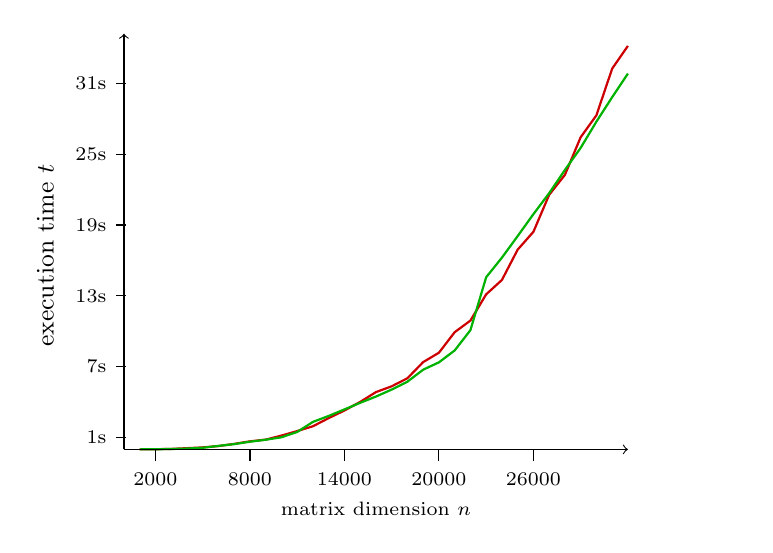
\begin{tikzpicture}[xscale=0.2,yscale=0.15]

\draw[color=red!80!black,thick] plot[id="magma"] coordinates {( 1,  0.0010) ( 2,  0.0140) ( 3,  0.0400) ( 4,  0.1027) ( 5,  0.1678) ( 6,  0.2814) ( 7,  0.4653) ( 8,  0.6813) ( 9,  0.8267) (10,  1.1692) (11,  1.5508) (12,  1.9600) (13,  2.6482) (14,  3.2920) (15,  4.0200) (16,  4.8500) (17,  5.3420) (18,  6.0233) (19,  7.3917) (20,  8.1840) (21,  9.9229) (22, 10.9067) (23, 13.1267) (24, 14.3450) (25, 16.9114) (26, 18.4225) (27, 21.5550) (28, 23.2440) (29, 26.4300) (30, 28.2850) (31, 32.2360) (32, 34.1620) } node[color=white] at (36.2, 34) {\small Magma};

\draw[thick,color=green!70!black] plot[id="M4RI"] coordinates {( 1,  0.0017) ( 2,  0.0102) ( 3,  0.0330) ( 4,  0.0699) ( 5,  0.1376) ( 6,  0.2953) ( 7,  0.4445) ( 8,  0.6496) ( 9,  0.8168) (10,  1.0241) (11,  1.4769) (12,  2.3285) (13,  2.8322) (14,  3.3850) (15,  3.9430) (16,  4.4731) (17,  5.0667) (18,  5.7327) (19,  6.7476) (20,  7.3711) (21,  8.3751) (22, 10.0966) (23, 14.5769) (24, 16.2330) (25, 18.0611) (26, 19.9190) (27, 21.6914) (28, 23.6595) (29, 25.5283) (30, 27.7492) (31, 29.8189) (32, 31.8200)} node[color=white] at (35.5,30) {\small M4RI};


  \draw[->] (-0.0,-0.0) -- (32.0,-0.0);
  \draw[->] (0,-0.0) -- (0,35.2);
  \draw (-5,16.4) node[rotate=90] {\small execution time $t$};

  \foreach \y in {1,7,...,34}
  \draw (0.1,\y) -- (-0.5,\y) node[anchor=east] {\scriptsize \y s};

  \foreach \x in {2,8,...,31} 
  \draw (\x,-1.0) -- (\x,0.0); 

\node at(2,-2.5) {\scriptsize 2000};
\node at(8,-2.5) {\scriptsize 8000};
\node at(14,-2.5) {\scriptsize 14000};
\node at(20,-2.5) {\scriptsize 20000};
\node at(26,-2.5) {\scriptsize 26000};

 \draw (16,-5.0) node {\scriptsize matrix dimension $n$};
\end{tikzpicture}
 %\includegraphics[width=0.8\textwidth]{benchmarketing-Multiplication-Magma-Sage.pdf}
\caption{2.66~Ghz Intel i7, 4GB RAM}
\end{figure}
\end{frame}

\begin{frame}
\frametitle{Work-in-Progress: Small Matrices}

M4RI is efficient for large matrices, but not so for small matrices. But there is work under way by Carlo Wood to fix this.

\begin{table}
\begin{tabular}{|l|l|l|}
\hline
 & Emmanuel & M4RI \\ 
\hline
transpose & 4.9064 $\mu s$ & 5.3642 $\mu s$ \\
copy      & 0.2019 $\mu s$ & 0.2674 $\mu s$ \\
add       & 0.2533 $\mu s$ & \textbf{\hlt 0.7503} $\mu s$ \\
mul       & 0.2535 $\mu s$ & 0.4472 $\mu s$ \\
\hline
\end{tabular}
\caption{$64 \times 64$ matrices (\texttt{matops.c})}
\end{table}

\begin{block}{Note}
One performance bottleneck is that our matrix structure is much more complicated than Emmanuel's. 
\end{block}
\end{frame}

\begin{frame}
\frametitle{Results: Multiplication Revisited}
\begin{figure}[h]
 \centering
 \includegraphics[width=0.8\textwidth]{benchmarketing-Multiplication-optimal.pdf}
\caption{2.66~Ghz Intel i7, 4GB RAM}
\end{figure}
\end{frame}

\subsection{Elimination}

\begin{frame}[allowframebreaks]
\frametitle{PLE Decomposition}

\begin{tabular}{ll}
\begin{minipage}{0.4\textwidth}
\begin{center}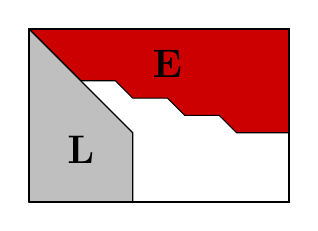
\begin{tikzpicture}[scale=0.22]
\draw[fill=white] (0,0) -- (0,10) -- (15,10) -- (15, 0) -- (0,0);
\draw[fill=red!80!black] (0,10) -- (3,7) -- (5,7) -- (6,6) -- (8,6) -- (9,5) -- (11,5) -- (12,4) -- (15,4) -- (15,10) -- (0,10);
\draw[fill=lightgray] (0,10) -- (6,4)  -- (6,0) -- (0,0) -- (0,10);

\draw[thick] (0,0) -- (0,10) -- (15,10) -- (15, 0) -- (0,0);
\node at (8,8) {\Large $\mathbf{E}$};
\node at (3,3) {\Large $\mathbf{L}$};
\end{tikzpicture}\end{center}
\end{minipage} & 
\begin{minipage}{0.5\textwidth}
\begin{definition}[PLE]
Let $A$ be a $m\times n$ matrix over a field $K$. A PLE decomposition of $A$ is
a triple of matrices $P,L$ and $E$ such that $P$ is a $m\times m$ permutation
matrix, $L$ is a unit lower triangular matrix, and $E$ is a $m\times n$ matrix
in row-echelon form, and $$A=PLE.$$
\end{definition}
\end{minipage}
\end{tabular}

\vspace{0.5cm}

PLE decomposition can be in-place, that is $L$ and $E$ are stored in $A$ and $P$ is stored as an $m$-vector.

\framebreak

From the PLE decomposition we can 
\begin{itemize}
 \item read the rank $r$,
 \item read the row rank profile (pivots),
 \item compute the null space,
 \item solve $y = Ax$ for $x$ and
 \item compute the (reduced) row echelon form.
\end{itemize}

\begin{thebibliography}{}
\bibitem{jeannerod-pernet-storjohann:cup2012}
C.-P. Jeannerod, C.~Pernet, and A.~Storjohann.
\newblock Rank-profile revealing {G}aussian elimination and the {CUP} matrix
  decomposition.
\newblock {\em {\tt arXiv:1112.5717}}, 35 pages, 2012.
 \end{thebibliography}


\end{frame}

\begin{frame}[allowframebreaks]
\frametitle{Block Recursive PLE Decomposition $\ord{n^{\omega}}$}

% Write $$A = \left(\begin{array}{cc} A_W & A_E\end{array}\right) = \left(\begin{array}{cc} A_{NW} & A_{NE}\\ A_{SW} & A_{SE}\end{array}\right)$$
% 
% Main steps:
% 
% \begin{enumerate}
% 
% \item Call PLE on $A_W$
% \item Apply row permutation to $A_E$
% \item $L_{NW} \leftarrow$ the lower left triangular matrix in $A_{NW}$
% \item $A_{NE} \leftarrow L_{NW}^{-1} \times A_{NE}$
% \item $A_{SE} \leftarrow A_{SE} + A_{SW} \times A_{NE}$
% \item Call PLE on $A_{SE}$
% \item Apply row permutation to $A_{SW}$
% \item Compress $L$
% \end{enumerate}
% 
% \framebreak
\vspace{-1.3em}
\begin{center}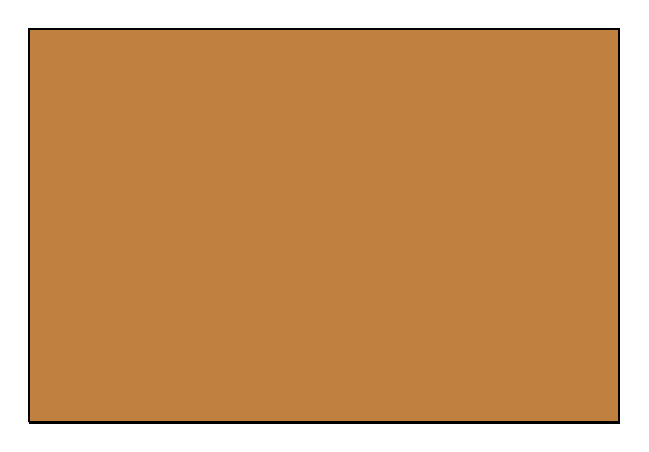
\begin{tikzpicture}[scale=0.5]
\draw[fill=brown] (0,0) -- (0,10) -- (15,10) -- (15, 0) -- (0,0);
\draw[thick] (0,0) -- (0,10) -- (15,10) -- (15, 0) -- (0,0);
\end{tikzpicture}\end{center}

\framebreak

\begin{center}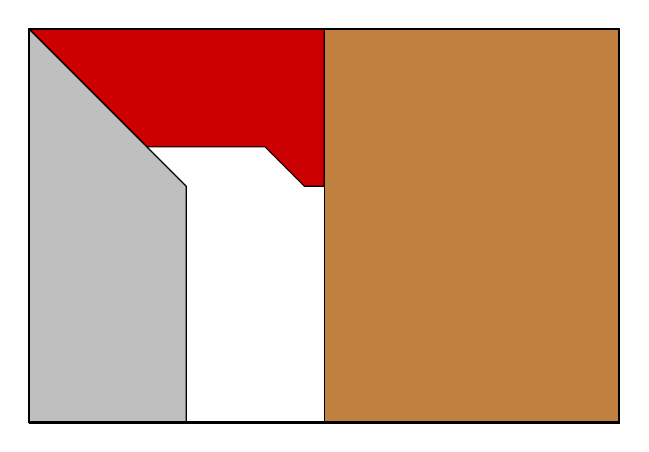
\begin{tikzpicture}[scale=0.5]
\draw[fill=brown] (0,0) -- (0,10) -- (15,10) -- (15, 0) -- (0,0);
\draw[fill=white] (0,0) --(0,10) -- (7.5,10) -- (7.5,0) -- (0,0);
\draw[fill=red!80!black] (0,10) -- (3,7) -- (6,7) -- (7,6) -- (7.5,6) -- (7.5,10) -- (0,10);
\draw[fill=lightgray] (0,10) -- (4,6) -- (4,0) -- (0,0) -- (0,10);
\draw[thick] (0,0) -- (0,10) -- (15,10) -- (15, 0) -- (0,0);
\end{tikzpicture}\end{center}

\framebreak

\begin{center}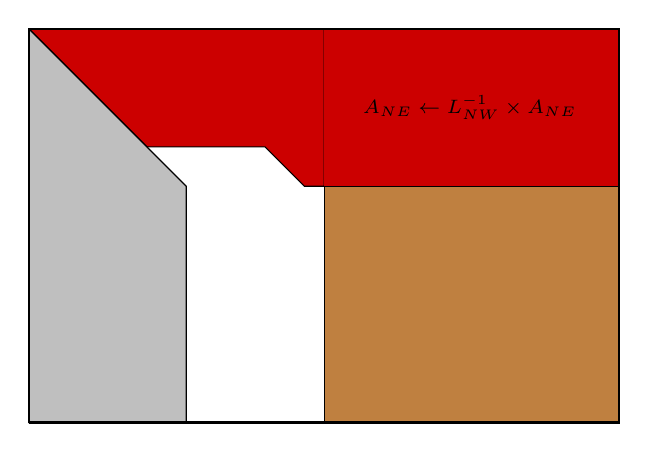
\begin{tikzpicture}[scale=0.5]
\draw[fill=brown] (0,0) -- (0,10) -- (15,10) -- (15, 0) -- (0,0);
\draw[fill=white] (0,0) --(0,10) -- (7.5,10) -- (7.5,0) -- (0,0);
\draw[fill=red!80!black] (0,10) -- (3,7) -- (6,7) -- (7,6) -- (7.5,6) -- (7.5,10) -- (0,10);
\draw[fill=lightgray] (0,10) -- (4,6) -- (4,0) -- (0,0) -- (0,10);
\draw[fill=red!80!black] (7.5,10) -- (15,10) -- (15,6) -- (7.5,6);
\node at (11.2,8) {\scriptsize $A_{NE} \leftarrow L_{NW}^{-1} \times A_{NE}$};
\draw[thick] (0,0) -- (0,10) -- (15,10) -- (15, 0) -- (0,0);
\end{tikzpicture}\end{center}

\framebreak

\begin{center}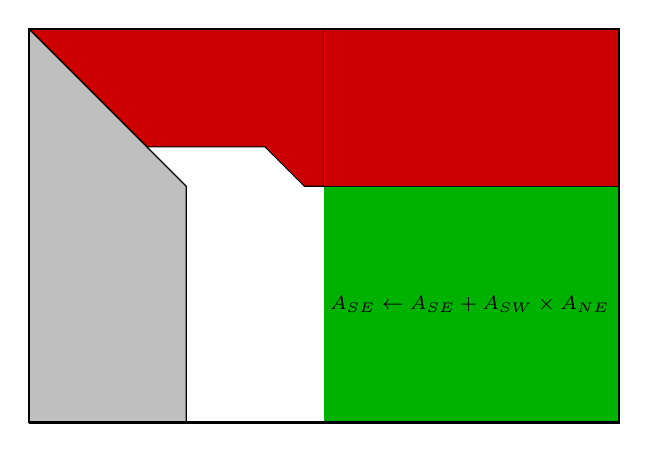
\begin{tikzpicture}[scale=0.5]
\draw[fill=brown] (0,0) -- (0,10) -- (15,10) -- (15, 0) -- (0,0);
\draw[fill=white] (0,0) --(0,10) -- (7.5,10) -- (7.5,0) -- (0,0);
\draw[fill=red!80!black] (0,10) -- (3,7) -- (6,7) -- (7,6) -- (7.5,6) -- (7.5,10) -- (0,10);
\draw[fill=lightgray] (0,10) -- (4,6) -- (4,0) -- (0,0) -- (0,10);
\draw[fill=red!80!black] (7.5,10) -- (15,10) -- (15,6) -- (7.5,6);
\draw[fill=green!70!black] (7.5,6) -- (15,6) -- (15,0) -- (7.5,0);
\node at (11.2,3) {\begin{scriptsize}$A_{SE} \leftarrow A_{SE} + A_{SW} \times A_{NE}$\end{scriptsize}};
\draw[thick] (0,0) -- (0,10) -- (15,10) -- (15, 0) -- (0,0);
\end{tikzpicture}\end{center}

\framebreak

\begin{center}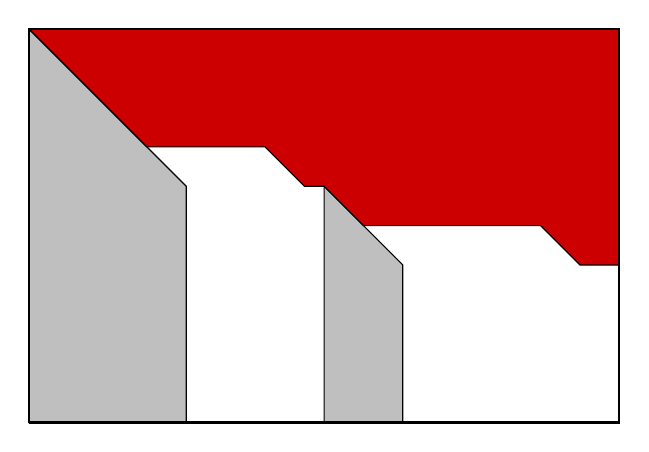
\begin{tikzpicture}[scale=0.5]
\draw[fill=white] (0,0) -- (0,10) -- (15,10) -- (15, 0) -- (0,0);
\draw[fill=lightgray] (0,10) -- (4,6) -- (4,0) -- (0,0) -- (0,10);
\draw[fill=lightgray] (7.5,6) -- (9.5,4) -- (9.5,0) -- (7.5,0) -- (7.5,6);
\draw[fill=red!80!black] (0,10) -- (3,7) -- (6,7) -- (7,6) -- (7.5,6) -- (8.5,5) -- (10,5) -- (13,5) -- (14,4) -- (15,4) -- (15,6) -- (15,10) -- (0,10);
\draw[thick] (0,0) -- (0,10) -- (15,10) -- (15, 0) -- (0,0);
\end{tikzpicture}\end{center}

\framebreak

\begin{center}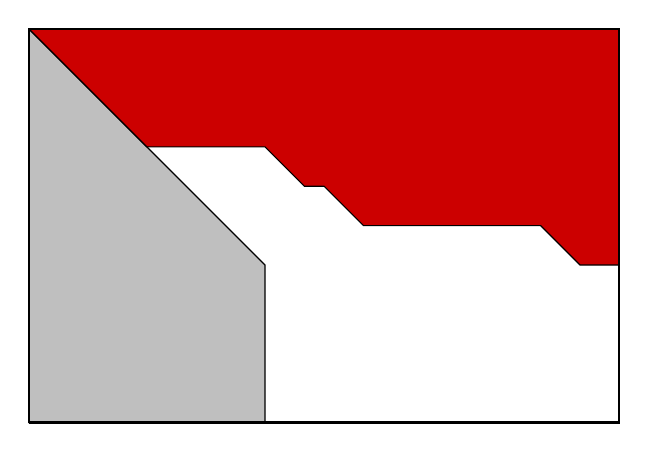
\begin{tikzpicture}[scale=0.5]
\draw[fill=white] (0,0) -- (0,10) -- (15,10) -- (15, 0) -- (0,0);
\draw[fill=lightgray] (0,10) -- (6,4) -- (6,0) -- (0,0) -- (0,10);
\draw[fill=red!80!black] (0,10) -- (3,7) -- (6,7) -- (7,6) -- (7.5,6) -- (8.5,5) -- (10,5) -- (13,5) -- (14,4) -- (15,4) -- (15,6) -- (15,10) -- (0,10);
\draw[thick] (0,0) -- (0,10) -- (15,10) -- (15, 0) -- (0,0);
\end{tikzpicture}\end{center}

\end{frame}

\begin{frame}[allowframebreaks,fragile]
\frametitle{Block Iterative PLE Decomposition} 

We need an efficient base case for PLE Decomposition

\begin{itemize}
 \item block recursive PLE decomposition gives rise to a block iterative PLE decomposition
 \item choose blocks of size $k = \log n$ and use M4RM for the ``update'' multiplications
 \item this gives a complexity $\ord{n^3 / \log n}$
\end{itemize}

% \begin{itemize}
%  \item this is an alternative way of looking at the M4RI algorithm or its PLE decomposition equivalent (``MMPF'')
%  \item M4RI is more cache friendly than straight block iterative PLE decomposition, so we adapt it PLE using M4RI ideas
% \end{itemize}

\framebreak

\begin{center}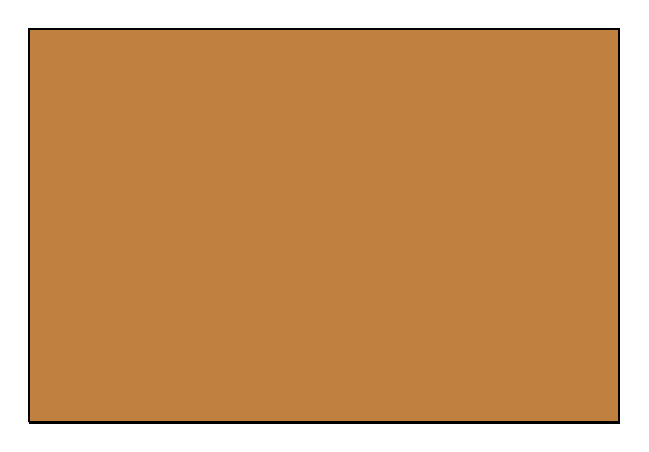
\begin{tikzpicture}[scale=0.5]
\draw[fill=brown] (0,0) -- (0,10) -- (15,10) -- (15, 0) -- (0,0);
\draw[thick] (0,0) -- (0,10) -- (15,10) -- (15, 0) -- (0,0);
\end{tikzpicture}\end{center}

\framebreak

\begin{center}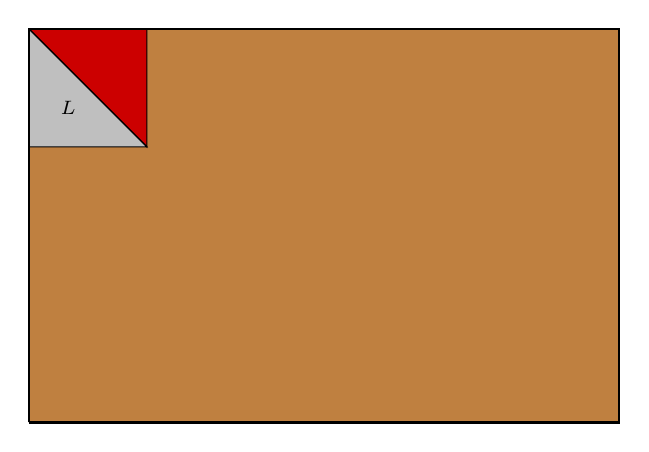
\begin{tikzpicture}[scale=0.5]
\draw[fill=brown] (0,0) -- (0,10) -- (15,10) -- (15, 0) -- (0,0);
\draw[fill=red!80!black] (0,10) -- (3,7) -- (3,10) -- (0,10);
\draw[fill=lightgray] (0,10) -- (3,7)  -- (0,7) -- (0,10);
\node at (1,8.0) {\scriptsize $L$};
\draw[thick] (0,0) -- (0,10) -- (15,10) -- (15, 0) -- (0,0);
\end{tikzpicture}\end{center}

\framebreak

\begin{center}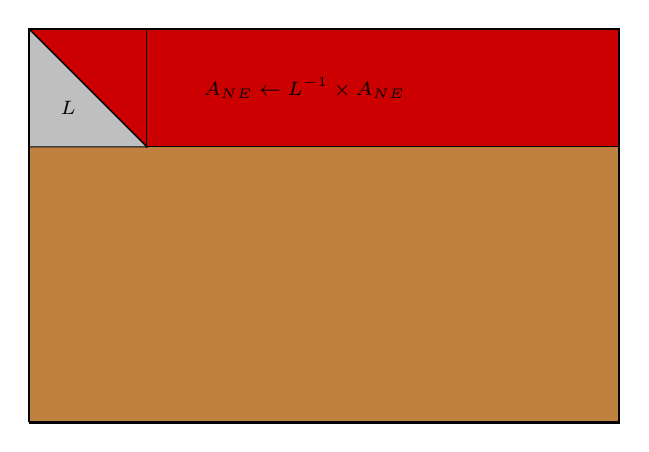
\begin{tikzpicture}[scale=0.5]
\draw[fill=brown] (0,0) -- (0,10) -- (15,10) -- (15, 0) -- (0,0);
\draw[fill=red!80!black] (0,10) -- (3,7) -- (3,10) -- (0,10);
\draw[fill=red!80!black] (3,10) -- (3,7) -- (15,7) -- (15,10) -- (3,10);
\node at (7,8.5) {\scriptsize $A_{NE} \leftarrow L^{-1} \times A_{NE}$};
\draw[fill=lightgray] (0,10) -- (3,7)  -- (0,7) -- (0,10);
\node at (1,8.0) {\scriptsize $L$};
\draw[thick] (0,0) -- (0,10) -- (15,10) -- (15, 0) -- (0,0);
\end{tikzpicture}\end{center}

\framebreak

\begin{center}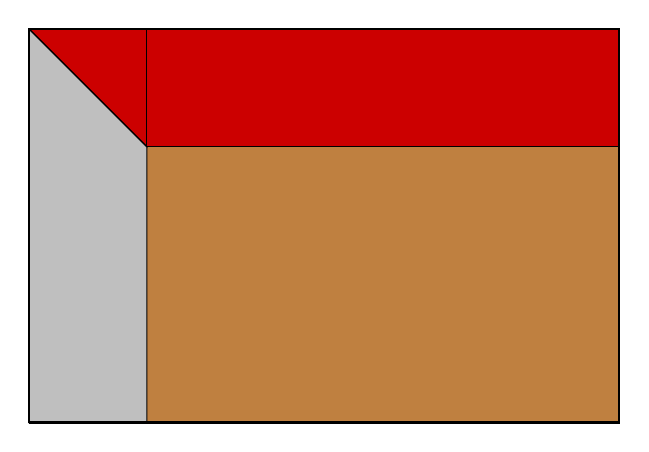
\begin{tikzpicture}[scale=0.5]
\draw[fill=brown] (0,0) -- (0,10) -- (15,10) -- (15, 0) -- (0,0);
\draw[fill=red!80!black] (0,10) -- (3,7) -- (3,10) -- (0,10);
\draw[fill=red!80!black] (3,10) -- (3,7) -- (15,7) -- (15,10) -- (3,10);
\draw[fill=lightgray] (0,10) -- (3,7)  -- (3,0) -- (0,0) -- (0,10);
\draw[thick] (0,0) -- (0,10) -- (15,10) -- (15, 0) -- (0,0);
\end{tikzpicture}\end{center}

\framebreak

\begin{center}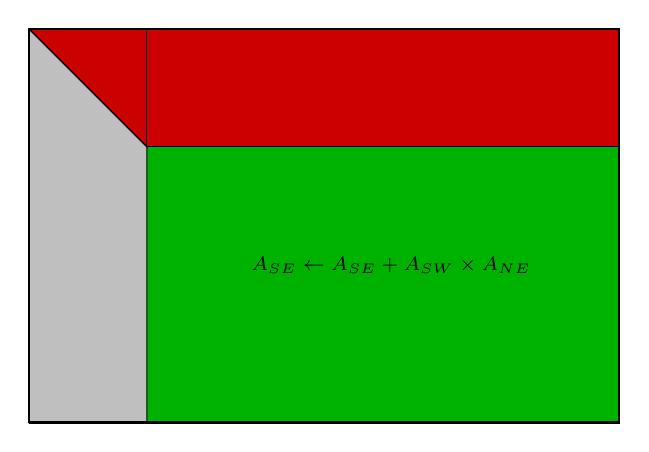
\begin{tikzpicture}[scale=0.5]
\draw[fill=green!70!black] (0,0) -- (0,10) -- (15,10) -- (15, 0) -- (0,0);
\draw[fill=red!80!black] (0,10) -- (3,7) -- (3,10) -- (0,10);
\draw[fill=red!80!black] (3,10) -- (3,7) -- (15,7) -- (15,10) -- (3,10);
\draw[fill=lightgray] (0,10) -- (3,7)  -- (3,0) -- (0,0) -- (0,10);
\node at (9.2,4) {\begin{scriptsize}$A_{SE} \leftarrow A_{SE} + A_{SW} \times A_{NE}$\end{scriptsize}};
\draw[thick] (0,0) -- (0,10) -- (15,10) -- (15, 0) -- (0,0);
\end{tikzpicture}\end{center}

\framebreak

\begin{center}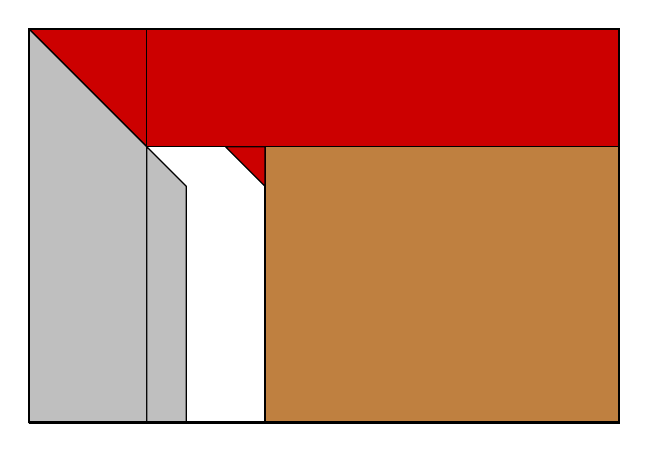
\begin{tikzpicture}[scale=0.5]
\draw[fill=brown] (0,0) -- (0,10) -- (15,10) -- (15, 0) -- (0,0);
\draw[fill=red!80!black] (0,10) -- (3,7) -- (3,10) -- (0,10);
\draw[fill=red!80!black] (3,10) -- (3,7) -- (15,7) -- (15,10) -- (3,10);
\draw[fill=lightgray] (0,10) -- (3,7)  -- (3,0) -- (0,0) -- (0,10);
\draw[fill=white] (3,7) -- (3,0) -- (6,0) -- (6,7) -- (3,7);
\draw[fill=red!80!black] (5,7) -- (6,6) -- (6,7) -- (5,7);
\draw[fill=lightgray] (3,7) -- (4,6) -- (4,0) -- (3,0) -- (3,7);
\draw[thick] (0,0) -- (0,10) -- (15,10) -- (15, 0) -- (0,0);
\end{tikzpicture}\end{center}

\framebreak

\begin{center}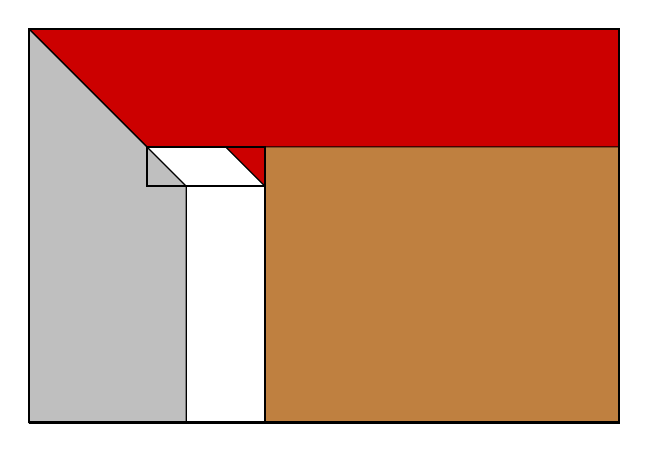
\begin{tikzpicture}[scale=0.5]
\draw[fill=brown] (0,0) -- (0,10) -- (15,10) -- (15, 0) -- (0,0);
\draw[fill=white] (3,7) -- (3,0) -- (6,0) -- (6,7) -- (3,7);
\draw[fill=red!80!black] (0,10) -- (3,7) -- (5,7) -- (6,6) -- (6,7) -- (15,7) -- (15,10) -- (0,10);
\draw[fill=lightgray] (0,10) -- (4,6)  -- (4,0) -- (0,0) -- (0,10);
\draw[thick,color=black] (3,7) -- (6,7) -- (6,6) -- (3,6) -- (3,7);
\draw[thick] (0,0) -- (0,10) -- (15,10) -- (15, 0) -- (0,0);
\end{tikzpicture}\end{center}

\framebreak

\begin{center}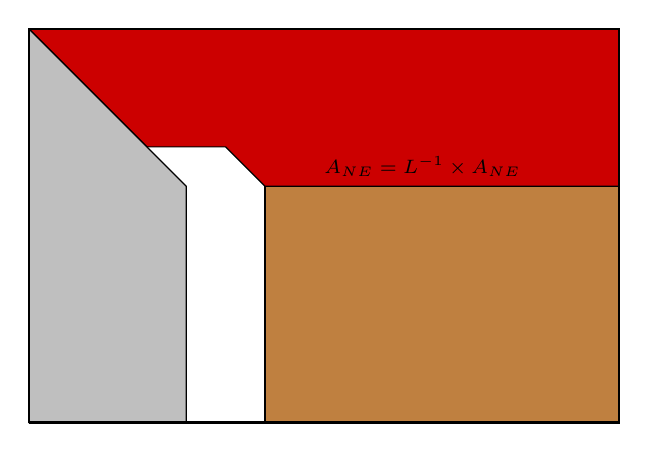
\begin{tikzpicture}[scale=0.5]
\draw[fill=brown] (0,0) -- (0,10) -- (15,10) -- (15, 0) -- (0,0);
\draw[fill=white] (3,7) -- (3,0) -- (6,0) -- (6,7) -- (3,7);
\draw[fill=red!80!black] (0,10) -- (3,7) -- (5,7) -- (6,6) --(15,6) -- (15,10) -- (0,10);
\draw[fill=lightgray] (0,10) -- (4,6)  -- (4,0) -- (0,0) -- (0,10);
\node at (10,6.5) {\scriptsize $A_{NE} = L^{-1} \times A_{NE}$};
\draw[thick] (0,0) -- (0,10) -- (15,10) -- (15, 0) -- (0,0);
\end{tikzpicture}\end{center}

\framebreak

\begin{center}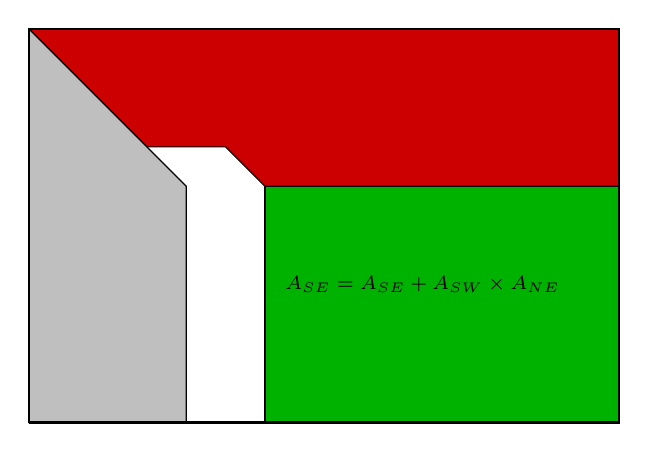
\begin{tikzpicture}[scale=0.5]
\draw[fill=green!70!black] (0,0) -- (0,10) -- (15,10) -- (15, 0) -- (0,0);
\draw[fill=white] (3,7) -- (3,0) -- (6,0) -- (6,7) -- (3,7);
\draw[fill=red!80!black] (0,10) -- (3,7) -- (5,7) -- (6,6) --(15,6) -- (15,10) -- (0,10);
\draw[fill=lightgray] (0,10) -- (4,6)  -- (4,0) -- (0,0) -- (0,10);
\node at (10,3.5) {\scriptsize $A_{SE} = A_{SE} + A_{SW} \times A_{NE}$};
\draw[thick] (0,0) -- (0,10) -- (15,10) -- (15, 0) -- (0,0);
\end{tikzpicture}\end{center}

\framebreak

\begin{center}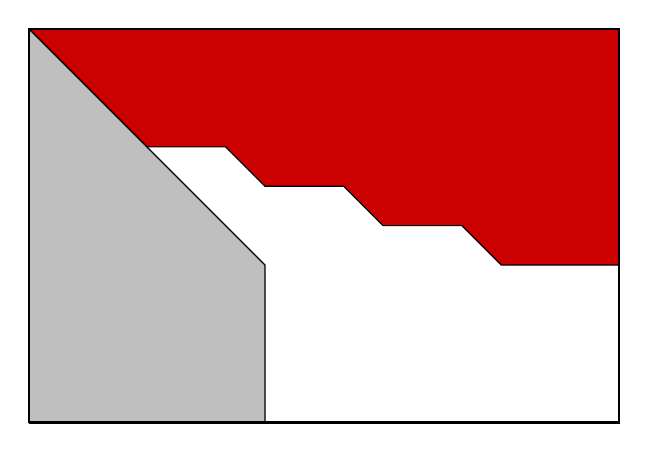
\begin{tikzpicture}[scale=0.5]
\draw[fill=white] (0,0) -- (0,10) -- (15,10) -- (15, 0) -- (0,0);
\draw[fill=red!80!black] (0,10) -- (3,7) -- (5,7) -- (6,6) -- (8,6) -- (9,5) -- (11,5) -- (12,4) -- (15,4) -- (15,10) -- (0,10);
\draw[fill=lightgray] (0,10) -- (6,4)  -- (6,0) -- (0,0) -- (0,10);

\draw[thick] (0,0) -- (0,10) -- (15,10) -- (15, 0) -- (0,0);
\end{tikzpicture}\end{center}

\end{frame}


\begin{frame}
\frametitle{Performance: Reduced Row Echelon Form}

\begin{figure}
 \centering
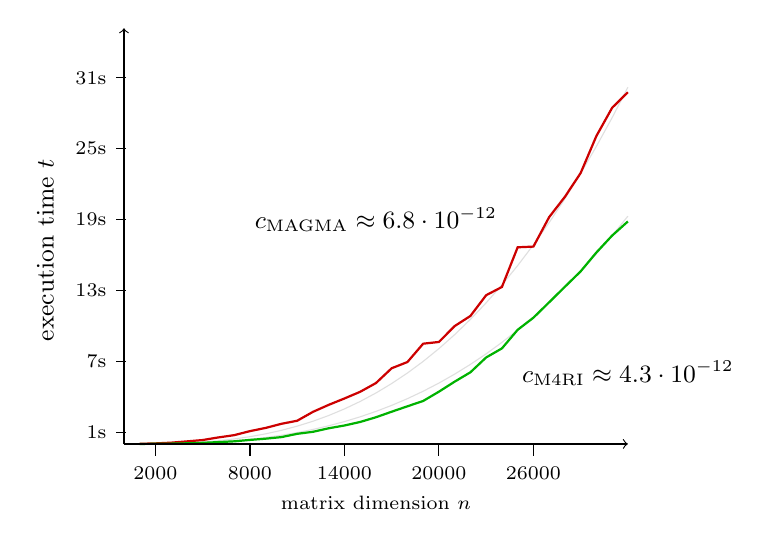
\begin{tikzpicture}[xscale=0.2,yscale=0.15]

\draw[color=lightgray, opacity=0.5] plot[id="magma clean"] coordinates {(0, 0.0) (1, 0.0017971059367291376) (2, 0.012579741557103966) (3, 0.039266517121090756) (4, 0.088058190899727759) (5, 0.16475194898605744) (6, 0.2748656198476353) (7, 0.42370522647991293) (8,0.6164073362980943) (9, 0.85796798914771188) (10, 1.1532636429024021) (11, 1.5070669968292192) (12, 1.924059338933447) (13, 2.4088404305686857) (14, 2.9659365853593904) (15, 3.5998073866299554) (16, 4.3148513540866604) (17, 5.1154107834503844) (18, 6.0057759240339834) (19, 6.9901886185299951) (20, 8.0728455003168147) (21, 9.2579008225583284) (22, 10.549468977804535) (23, 11.95162675508465) (24, 13.46841537253413) (25, 15.103842316667796) (26, 16.861883013980801) (27, 18.746482356256415) (28, 20.761556097515736) (29, 22.910992137762481) (30, 25.198651706409688) (31, 27.628370456414309) (32, 30.203959478606624)};

\draw[color=red!80!black,thick] plot[id="magma"] coordinates {( 1,  0.0126) ( 2,  0.0475) ( 3,  0.1097) ( 4,  0.2186) ( 5,  0.3323) ( 6,  0.5542) ( 7,  0.7450) ( 8,  1.0870) ( 9,  1.3586) (10,  1.7071) (11,  1.9658) (12,  2.7172) (13,  3.3110) (14,  3.8500) (15,  4.4178) (16,  5.1548) (17,  6.4100) (18,  6.9372) (19,  8.4892) (20,  8.6364) (21,  9.9820) (22, 10.8379) (23, 12.5963) (24, 13.2912) (25, 16.6520) (26, 16.7100) (27, 19.2075) (28, 20.9277) (29, 22.9422) (30, 26.0771) (31, 28.4657) (32, 29.7840)} node[color=white] at (36.2, 29) {\small Magma};

\draw[color=lightgray,opacity=0.5] plot[id="M4RI clean"] coordinates {(0, 0.0) (1, 0.0011477373960293543) (2, 0.0080341617722054816) (3, 0.025077903973612779) (4, 0.056239132405438368) (5, 0.10522027057802702) (6, 0.17554532781528948) (7, 0.27060304202722091) (8, 0.39367392683806862) (9, 0.54794874671284044) (10, 0.73654189404618919) (11, 0.96250149489281478) (12, 1.2288172947070264) (13, 1.5384269712352709) (14, 1.8942212941905465) (15, 2.2990484153971305) (16, 2.7557174878664803) (17, 3.2670017566709149) (18, 3.8356412269898832) (19, 4.4643449886921545) (20, 5.1557932583233246) (21, 5.9126391859349932) (22, 6.7375104642497039) (23, 7.6330107701731515) (24, 8.6017210629491849) (25, 9.6462007588276411) (26, 10.768988798646898) (27, 11.972604621985008) (28, 13.259549059333827) (29, 14.632305151973831) (30, 16.093338907779913) (31, 17.645099999999996) (32, 19.290022415065362)};

\draw[thick,color=green!70!black] plot[id="M4RI"] coordinates {( 1,  0.0025) ( 2,  0.0114) ( 3,  0.0287) ( 4,  0.0548) ( 5,  0.0960) ( 6,  0.1571) ( 7,  0.2229) ( 8,  0.3420) ( 9,  0.4464) (10,  0.5806) (11,  0.8585) (12,  1.0288) (13,  1.3281) (14,  1.5625) (15,  1.8626) (16,  2.2606) (17,  2.7302) (18,  3.1889) (19,  3.6416) (20,  4.4266) (21,  5.2763) (22,  6.0677) (23,  7.3262) (24,  8.0905) (25,  9.6663) (26, 10.6887) (27, 11.9967) (28, 13.3112) (29, 14.6136) (30, 16.2135) (31, 17.6451) (32, 18.8412)} node[color=white] at (35.5,19) {\small M4RI};


\draw[->] (-0.0,-0.0) -- (32.0,-0.0);
\draw[->] (0,-0.0) -- (0,35.2);
\draw (-5,16.4) node[rotate=90] {\small execution time $t$};

\foreach \y in {1,7,...,34}
  \draw (0.1,\y) -- (-0.5,\y) node[anchor=east] {\scriptsize \y s};

\foreach \x in {2,8,...,31} 
  \draw (\x,-1.0) -- (\x,0.0); 

\node at(2,-2.5) {\scriptsize 2000};
\node at(8,-2.5) {\scriptsize 8000};
\node at(14,-2.5) {\scriptsize 14000};
\node at(20,-2.5) {\scriptsize 20000};
\node at(26,-2.5) {\scriptsize 26000};
\draw (16,-5.0) node {\scriptsize matrix dimension $n$};

\node at (32,6) {\small $c_{\textnormal{M4RI}} \approx 4.3 \cdot 10^{-12}$};
\node at (16,19) {\small $c_{\textnormal{MAGMA}} \approx 6.8 \cdot 10^{-12}$};

\end{tikzpicture}
\caption{2.66~Ghz Intel i7, 4GB RAM}
\end{figure}

\end{frame}
 
\begin{frame}
\frametitle{Performance: Row Echelon Form}

Using one core -- on sage.math -- we can compute the echelon form of a \(500,000 \times 500,000\) dense random matrix  over $\mathbb{F}_2$ in \[9711\textnormal{ seconds }= 2.7\textnormal{ hours } (c \approx 10^{-12}).\] 

Using four cores decomposition we can compute the echelon form of a random dense \(500,000 \times 500,000\) matrix in \[3806\textnormal{ seconds }= 1.05\textnormal{ hours.}\]

\end{frame}

\subsection{Gröbner Basis Computations}

\begin{frame}[fragile,allowframebreaks]
\frametitle{Caveat: Sensitivity to Sparsity}

\begin{figure}[htbp]
\begin{center}
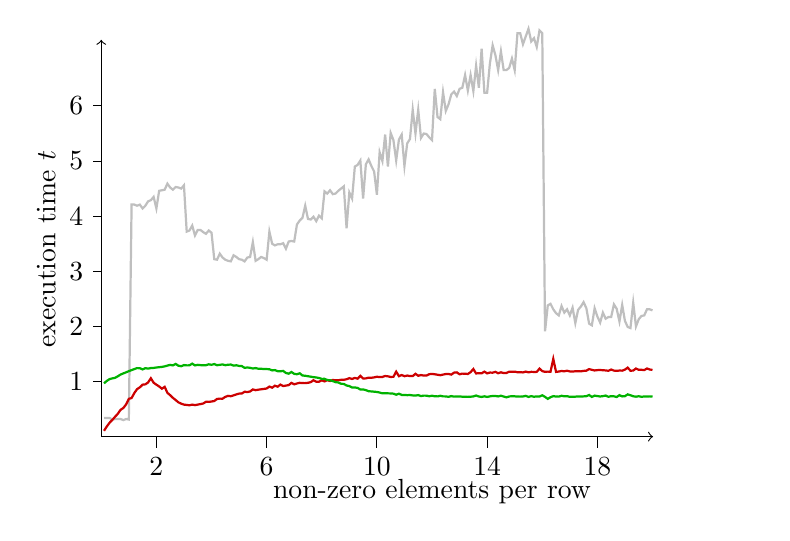
\begin{tikzpicture}[xscale=0.035,yscale=0.7]
  \draw[->] (-0.0,-0.0) -- (200.2,-0.0);
  \draw[->] (0,-0.0) -- (0,7.2);
  \draw (-20,3.4) node[rotate=90] {execution time $t$};

  \foreach \y in {1,...,6}
  \draw (0.1,\y) -- (-3,\y) node[anchor=east] {\y};

  %ticks
  \draw (20,-0.0) -- (20,-0.2) node[anchor=north] {2};
  \draw (60,-0.0) -- (60,-0.2) node[anchor=north] {6};
  \draw (100,-0.0) -- (100,-0.2) node[anchor=north] {10};
  \draw (140,-0.0) -- (140,-0.2) node[anchor=north] {14};
  \draw (180,-0.0) -- (180,-0.2) node[anchor=north] {18};

  \draw (120,-1.0) node {non-zero elements per row};


  \draw[thick,color=lightgray] plot[id="magma"] coordinates {(1, 0.34000) (2, 0.34000) (3, 0.34000) (4, 0.31000) (5, 0.32000) (6, 0.32000) (7, 0.32000) (8, 0.30000) (9, 0.32000) (10, 0.31000) (11, 4.21000) (12, 4.21000) (13, 4.19000) (14, 4.21000) (15, 4.14000) (16, 4.19000) (17, 4.27000) (18, 4.29000) (19, 4.35000) (20, 4.14000) (21, 4.46000) (22, 4.47000) (23, 4.48000) (24, 4.59000) (25, 4.52000) (26, 4.48000) (27, 4.53000) (28, 4.52000) (29, 4.50000) (30, 4.56000) (31, 3.72000) (32, 3.74000) (33, 3.83000) (34, 3.65000) (35, 3.75000) (36, 3.75000) (37, 3.71000) (38, 3.68000) (39, 3.74000) (40, 3.70000) (41, 3.22000) (42, 3.21000) (43, 3.32000) (44, 3.25000) (45, 3.21000) (46, 3.19000) (47, 3.18000) (48, 3.29000) (49, 3.26000) (50, 3.22000) (51, 3.21000) (52, 3.18000) (53, 3.25000) (54, 3.26000) (55, 3.53000) (56, 3.19000) (57, 3.22000) (58, 3.26000) (59, 3.24000) (60, 3.21000) (61, 3.72000) (62, 3.50000) (63, 3.47000) (64, 3.49000) (65, 3.49000) (66, 3.51000) (67, 3.41000) (68, 3.54000) (69, 3.55000) (70, 3.54000) (71, 3.85000) (72, 3.92000) (73, 3.97000) (74, 4.19000) (75, 3.95000) (76, 3.94000) (77, 3.99000) (78, 3.91000) (79, 4.01000) (80, 3.96000) (81, 4.45000) (82, 4.41000) (83, 4.47000) (84, 4.40000) (85, 4.41000) (86, 4.46000) (87, 4.50000) (88, 4.54000) (89, 3.78000) (90, 4.43000) (91, 4.32000) (92, 4.90000) (93, 4.93000) (94, 5.01000) (95, 4.32000) (96, 4.94000) (97, 5.03000) (98, 4.91000) (99, 4.81000) (100, 4.39000) (101, 5.16000) (102, 5.00000) (103, 5.48000) (104, 4.90000) (105, 5.51000) (106, 5.38000) (107, 5.01000) (108, 5.39000) (109, 5.48000) (110, 4.91000) (111, 5.32000) (112, 5.40000) (113, 5.93000) (114, 5.50000) (115, 5.93000) (116, 5.42000) (117, 5.50000) (118, 5.49000) (119, 5.43000) (120, 5.38000) (121, 6.31000) (122, 5.80000) (123, 5.76000) (124, 6.25000) (125, 5.91000) (126, 6.03000) (127, 6.21000) (128, 6.26000) (129, 6.18000) (130, 6.31000) (131, 6.33000) (132, 6.56000) (133, 6.28000) (134, 6.56000) (135, 6.27000) (136, 6.73000) (137, 6.33000) (138, 7.04000) (139, 6.24000) (140, 6.24000) (141, 6.77000) (142, 7.10000) (143, 6.92000) (144, 6.65000) (145, 6.99000) (146, 6.65000) (147, 6.65000) (148, 6.69000) (149, 6.86000) (150, 6.65000) (151, 7.32000) (152, 7.32000) (153, 7.12000) (154, 7.26000) (155, 7.40000) (156, 7.17000) (157, 7.23000) (158, 7.07000) (159, 7.37000) (160, 7.32000) (161, 1.91000) (162, 2.38000) (163, 2.41000) (164, 2.31000) (165, 2.24000) (166, 2.20000) (167, 2.37000) (168, 2.25000) (169, 2.31000) (170, 2.20000) (171, 2.34000) (172, 2.06000) (173, 2.30000) (174, 2.36000) (175, 2.44000) (176, 2.33000) (177, 2.05000) (178, 2.02000) (179, 2.33000) (180, 2.18000) (181, 2.07000) (182, 2.25000) (183, 2.14000) (184, 2.17000) (185, 2.17000) (186, 2.40000) (187, 2.32000) (188, 2.09000) (189, 2.39000) (190, 2.10000) (191, 1.99000) (192, 1.97000) (193, 2.43000) (194, 2.00000) (195, 2.13000) (196, 2.19000) (197, 2.20000) (198, 2.31000) (199, 2.31000) (200, 2.29000)}  node[right,color=white] {Magma};

\draw[color=red!80!black,thick] plot[id="m4ri"] coordinates {(1, 0.106155) (2, 0.184164) (3, 0.251415) (4, 0.303108) (5, 0.360643) (6, 0.414627) (7, 0.486798) (8, 0.519742) (9, 0.583870) (10, 0.685364) (11, 0.701443) (12, 0.791403) (13, 0.862657) (14, 0.894982) (15, 0.943845) (16, 0.948925) (17, 0.983653) (18, 1.058876) (19, 0.978244) (20, 0.942851) (21, 0.910335) (22, 0.870607) (23, 0.903626) (24, 0.794898) (25, 0.751917) (26, 0.703680) (27, 0.664177) (28, 0.622128) (29, 0.598736) (30, 0.581246) (31, 0.575591) (32, 0.569314) (33, 0.581121) (34, 0.571415) (35, 0.581529) (36, 0.590549) (37, 0.602096) (38, 0.633154) (39, 0.631056) (40, 0.637458) (41, 0.647052) (42, 0.683402) (43, 0.690109) (44, 0.688369) (45, 0.721489) (46, 0.740237) (47, 0.733376) (48, 0.749635) (49, 0.766576) (50, 0.780792) (51, 0.782709) (52, 0.815303) (53, 0.808925) (54, 0.819675) (55, 0.856786) (56, 0.842952) (57, 0.852394) (58, 0.859198) (59, 0.866153) (60, 0.873672) (61, 0.908846) (62, 0.888298) (63, 0.924500) (64, 0.906349) (65, 0.944918) (66, 0.917566) (67, 0.926394) (68, 0.935242) (69, 0.976125) (70, 0.949351) (71, 0.964972) (72, 0.976726) (73, 0.971648) (74, 0.971378) (75, 0.976877) (76, 0.989472) (77, 1.023465) (78, 0.996700) (79, 0.996345) (80, 1.021938) (81, 1.002980) (82, 1.025406) (83, 1.009642) (84, 1.028584) (85, 1.022169) (86, 1.023683) (87, 1.031212) (88, 1.032265) (89, 1.041096) (90, 1.061411) (91, 1.046542) (92, 1.065558) (93, 1.052070) (94, 1.103617) (95, 1.054645) (96, 1.057528) (97, 1.070088) (98, 1.068171) (99, 1.075558) (100, 1.086820) (101, 1.081535) (102, 1.083108) (103, 1.100390) (104, 1.094615) (105, 1.083225) (106, 1.085532) (107, 1.179791) (108, 1.096924) (109, 1.118066) (110, 1.096977) (111, 1.108275) (112, 1.099314) (113, 1.098875) (114, 1.140278) (115, 1.104692) (116, 1.117734) (117, 1.107452) (118, 1.108677) (119, 1.133074) (120, 1.138049) (121, 1.131893) (122, 1.123428) (123, 1.115298) (124, 1.125756) (125, 1.136285) (126, 1.137816) (127, 1.125501) (128, 1.161839) (129, 1.166295) (130, 1.131556) (131, 1.143585) (132, 1.142175) (133, 1.137177) (134, 1.170231) (135, 1.226686) (136, 1.146127) (137, 1.152069) (138, 1.148524) (139, 1.179800) (140, 1.148448) (141, 1.162584) (142, 1.160667) (143, 1.176126) (144, 1.150629) (145, 1.167743) (146, 1.153145) (147, 1.155713) (148, 1.178170) (149, 1.176623) (150, 1.179899) (151, 1.168482) (152, 1.168863) (153, 1.165564) (154, 1.180034) (155, 1.167097) (156, 1.176009) (157, 1.174169) (158, 1.175008) (159, 1.235052) (160, 1.188697) (161, 1.176353) (162, 1.179927) (163, 1.178066) (164, 1.410760) (165, 1.175002) (166, 1.181250) (167, 1.190936) (168, 1.185536) (169, 1.195529) (170, 1.183506) (171, 1.179883) (172, 1.187214) (173, 1.184755) (174, 1.184619) (175, 1.193059) (176, 1.197349) (177, 1.225413) (178, 1.212423) (179, 1.201041) (180, 1.207087) (181, 1.208996) (182, 1.205363) (183, 1.201408) (184, 1.195647) (185, 1.217675) (186, 1.198349) (187, 1.193616) (188, 1.199563) (189, 1.197402) (190, 1.215841) (191, 1.252375) (192, 1.196108) (193, 1.199229) (194, 1.236302) (195, 1.212404) (196, 1.212873) (197, 1.207745) (198, 1.236736) (199, 1.218035) (200, 1.210933)} node[right,color=white] {M4RI};


\draw[color=green!70!black,thick] plot[id="ple"] coordinates {(1, 0.967001) (2, 1.011240) (3, 1.043532) (4, 1.057283) (5, 1.067011) (6, 1.094712) (7, 1.126642) (8, 1.147539) (9, 1.166968) (10, 1.188493) (11, 1.207241) (12, 1.226128) (13, 1.243596) (14, 1.242186) (15, 1.220430) (16, 1.242211) (17, 1.234236) (18, 1.244736) (19, 1.247406) (20, 1.254644) (21, 1.260065) (22, 1.265938) (23, 1.274927) (24, 1.289218) (25, 1.302123) (26, 1.292878) (27, 1.319090) (28, 1.286986) (29, 1.277622) (30, 1.298599) (31, 1.293035) (32, 1.293842) (33, 1.324919) (34, 1.292739) (35, 1.302995) (36, 1.297650) (37, 1.294314) (38, 1.295756) (39, 1.312144) (40, 1.304358) (41, 1.316395) (42, 1.296363) (43, 1.302899) (44, 1.310021) (45, 1.296868) (46, 1.305285) (47, 1.307949) (48, 1.288711) (49, 1.294765) (50, 1.283429) (51, 1.280192) (52, 1.248310) (53, 1.255100) (54, 1.248704) (55, 1.236663) (56, 1.243733) (57, 1.232309) (58, 1.231709) (59, 1.226472) (60, 1.226308) (61, 1.222957) (62, 1.201951) (63, 1.207814) (64, 1.187733) (65, 1.185693) (66, 1.192795) (67, 1.155630) (68, 1.142165) (69, 1.172876) (70, 1.138912) (71, 1.132558) (72, 1.149631) (73, 1.110075) (74, 1.104494) (75, 1.096257) (76, 1.088169) (77, 1.079330) (78, 1.073613) (79, 1.064443) (80, 1.047714) (81, 1.049457) (82, 1.027283) (83, 1.023933) (84, 1.008276) (85, 0.988839) (86, 0.983257) (87, 0.959266) (88, 0.956504) (89, 0.928407) (90, 0.917338) (91, 0.892135) (92, 0.892280) (93, 0.884687) (94, 0.854258) (95, 0.856597) (96, 0.844121) (97, 0.824273) (98, 0.820348) (99, 0.815931) (100, 0.810675) (101, 0.800143) (102, 0.785634) (103, 0.788427) (104, 0.785680) (105, 0.784312) (106, 0.780050) (107, 0.760630) (108, 0.779530) (109, 0.757411) (110, 0.757455) (111, 0.752751) (112, 0.755011) (113, 0.748248) (114, 0.744579) (115, 0.754171) (116, 0.736143) (117, 0.744608) (118, 0.743812) (119, 0.733087) (120, 0.741566) (121, 0.732432) (122, 0.730616) (123, 0.741013) (124, 0.730900) (125, 0.730208) (126, 0.722856) (127, 0.735323) (128, 0.726059) (129, 0.728209) (130, 0.728833) (131, 0.725145) (132, 0.725483) (133, 0.721675) (134, 0.724811) (135, 0.729282) (136, 0.746324) (137, 0.728213) (138, 0.720790) (139, 0.731694) (140, 0.720459) (141, 0.731025) (142, 0.738490) (143, 0.737890) (144, 0.729711) (145, 0.742782) (146, 0.727809) (147, 0.713109) (148, 0.729410) (149, 0.733000) (150, 0.731499) (151, 0.727514) (152, 0.726306) (153, 0.729044) (154, 0.740103) (155, 0.720986) (156, 0.734946) (157, 0.724087) (158, 0.730419) (159, 0.727758) (160, 0.750673) (161, 0.721864) (162, 0.685695) (163, 0.715466) (164, 0.735101) (165, 0.727639) (166, 0.726179) (167, 0.741733) (168, 0.732329) (169, 0.735057) (170, 0.721917) (171, 0.725240) (172, 0.725486) (173, 0.730473) (174, 0.727208) (175, 0.730838) (176, 0.733854) (177, 0.755746) (178, 0.720966) (179, 0.744222) (180, 0.736405) (181, 0.728481) (182, 0.735357) (183, 0.745696) (184, 0.722822) (185, 0.735396) (186, 0.731748) (187, 0.719136) (188, 0.752489) (189, 0.730183) (190, 0.734502) (191, 0.767001) (192, 0.751637) (193, 0.732539) (194, 0.725180) (195, 0.733402) (196, 0.722572) (197, 0.729101) (198, 0.728895) (199, 0.730496) (200, 0.729762)} node[right,color=white] {PLE};

\end{tikzpicture}
\caption{Gaussian elimination of $10,000 \times 10,000$ matrices on Intel 2.33GHz Xeon E5345 comparing Magma 2.17-12 and M4RI 20111004.}
\label{fig:sparse-m4ri}
\end{center}
\end{figure}

\framebreak

Why is that?
\begin{enumerate}
 \item These algorithms are designed to be \emph{rank sensitive} and they swap rows and columns. The latter is quite expensive.
 \item Searching for a pivot often requires to deal with single bits instead of complete words.
 \item We loose cache efficiency by doing less operations on those rows already in cache.
\end{enumerate}
\end{frame}

\begin{frame}[allowframebreaks,fragile]
\frametitle{New Project}
\begin{itemize}
 \item New repository for code optimised for Gröbner basis computations,
 \item supports timing of three algorithms (PLE, M4RI, GB) and
 \item reads 1-bit PNG images during execution,
 \item plotting of intermediate matrices.
\end{itemize}

\framebreak

\begin{lstlisting}
groebner

REQUIRED
  filename (1-bit PNG or JCF format)

OPTIONAL
  -w filename    write the processed matrix to a 1-bit PNG
  -c level       compression level for output
  -e algo        echelonize using algorithm 'algo'
  -r             compute the rank
  -v             write intermediate matrices when executing 
                 gb algorithm
\end{lstlisting}

\begin{block}{}
\centering \url{https://bitbucket.org/malb/m4ri-groebner}
\end{block}

\end{frame}

\begin{frame}[fragile,allowframebreaks]
\frametitle{Algorithm}

The implemented algorithm is very simple variant of \cite{faugere-lachatre:pasco2010,polybori}

\begin{thebibliography}{foobar}
\bibitem{faugere-lachatre:pasco2010} J.-C. Faug\`ere and S.~Lachartre.
\newblock {P}arallel {G}aussian {E}limination for {G}röbner bases computations in finite fields.
\newblock In {\em Proceedings of the 4th International Workshop on Parallel and Symbolic Computation}, pages 89--97, 2010.

\bibitem{polybori} M.\ Brickenstein and A.\ Dreyer.
\newblock {PolyBoRi}: A framework for {G}r{\"o}bner basis computations with {B}oolean polynomials.
\newblock In {\em Electronic Proceedings of MEGA 2007}, 2007.
\end{thebibliography}


\framebreak

\begin{lstlisting} 
  mzp_t *Q = mzp_init(n);
  rci_t r0 = mzd_analyse_gb(A, Q);

  for(rci_t i=0; i<r0; i++) {
    mzd_row_swap(A, i, Q->values[i]);
  }
  for(rci_t i=r0; i<MIN(m,n); i++) {
   if (Q->values[i] >= r0 && Q->values[i] < MIN(m,n))
     mzd_row_swap(A, i, Q->values[i]);
  }

  mzd_t *ANW = mzd_init_window(A,  0,  0, r0, r0);
  mzd_t *ASW = mzd_init_window(A, r0,  0,  m, r0);
  mzd_t *ANE = mzd_init_window(A,  0, r0, r0,  n);
  mzd_t *ASE = mzd_init_window(A, r0, r0,  m,  n);

  mzd_trsm_upper_left(ANW, ANE, 0);
  mzd_addmul(ASE, ASW, ANE, 0);

  mzd_set_ui(ANW,1);
  mzd_set_ui(ASW,0);

  r0 += mzd_echelonize_pluq(ASE, 0);
\end{lstlisting}
\end{frame}


\begin{frame}[allowframebreaks]
\frametitle{Example}
\begin{center}
\vspace{-1.2em}
\includegraphics[width=0.75\textwidth]{./hfe_25_5_echelonize_step_000.png}\\\framebreak
\includegraphics[width=0.75\textwidth]{./hfe_25_5_echelonize_step_001.png}\\\framebreak
\includegraphics[width=0.75\textwidth]{./hfe_25_5_echelonize_step_002.png}\\\framebreak
\includegraphics[width=0.75\textwidth]{./hfe_25_5_echelonize_step_003.png}\\\framebreak
\includegraphics[width=0.75\textwidth]{./hfe_25_5_echelonize_step_004.png}\\\framebreak
\includegraphics[width=0.75\textwidth]{./hfe_25_5_echelonize_step_005.png}\\\framebreak
 \end{center}
\end{frame}

\begin{frame}[allowframebreaks]
\frametitle{Results}


\begin{footnotesize}
\begin{center}
\begin{tabular}{|l|r|r|r|r|r|r||r|}
\hline
problem  & $m$ & $n$ &  dens. &  PLE & M4RI & GB & LELA\\
\hline        
HFE 25        &   12307 & 13508 & 0.076 &                1.0 &  {\color{pink} 0.5}&                  0.8 &   0.7\\
HFE 30        &   19907 & 29323 & 0.067 &                4.7 &  {\color{pink} 2.7}&                  4.7 &   5.4\\
HFE 35        &   29969 & 55800 & 0.059 &               19.3 &  {\color{pink} 9.2}&                 19.5 &  21.8\\
Mutant        &   26075 & 26407 & 0.184 &                5.7 &                3.9 &   {\color{pink}  2.1}&  10.9\\
n=24, m=26    &   37587 & 38483 & 0.038 &               20.6 &               21.0 &   {\color{pink} 19.3}&  10.1\\
n=24, m=26    &   37576 & 32288 & 0.040 &               18.6 &               28.4 &   {\color{pink} 17.0}&   4.5\\
SR(2,2,2,4) c &    5640 & 14297 & 0.003 &                0.4 &                0.2 &   {\color{pink}  0.1}&   1.0\\
SR(2,2,2,4) c &   13665 & 17394 & 0.013 &                2.1 &                3.0 &   {\color{pink}  2.0}&   4.0\\
SR(2,2,2,4) c &   11606 & 16282 & 0.035 &                1.9 &                4.4 &   {\color{pink}  1.5}&   2.2\\
SR(2,2,2,4)   &   13067 & 17511 & 0.008 &                1.9 &                2.0 &   {\color{pink}  1.3}&   3.4\\
SR(2,2,2,4)   &   12058 & 16662 & 0.015 &  {\color{pink} 1.5}&                1.9 &                  1.6 &   2.7\\
SR(2,2,2,4)   &  115834 &118589 & 0.003 &              528.2 &              578.5 &  {\color{pink} 522.9}&  95.0\\
\hline
\end{tabular}
\end{center}
\end{footnotesize}

\begin{block}{}
LELA does reduced row echelon forms, M4RI does not.
\end{block}


\end{frame}



\section{\texorpdfstring{$\F_{2^e}$}{F2E}}

\begin{frame}
\frametitle{The M4RIE Library}
\begin{itemize}
\item handles $\mathbb{F}_{2^e}$ for $2 \leq e \leq 10$; $e \leq 16$ planned.
\item available under the GPL Version 2 or later (GPLv2+)
\item provides basic arithmetic (addition, equality testing, stacking, augmenting, sub-matrices, randomisation, etc.)
\item implements asymptotically fast multiplication
\item implements asymptotically fast elimination
\item Linux, Mac OS X (x86 and PPC), OpenSolaris, and Windows (Cygwin)
\end{itemize}

\begin{block}{}
\centering
\url{http://m4ri.sagemath.org} 
\end{block}
\end{frame}

\begin{frame}[allowframebreaks]
\frametitle{Representation of Elements} 


Elements in $\F_{2^e} \cong \F_2[x]/f$ can be written as $$a_0 \alpha^0 + a_1 \alpha^1 + \dots + a_{e-1} \alpha^{e-1}.$$

\vspace{1em}

We identify the bitstring $a_0,\dots,a_{e-1}$ with
 \begin{itemize}
  \item the element $\sum_{i=0}^{e-1} a_i \alpha^i \in \F_{2^e}$ and
  \item the integer $\sum_{i=0}^{e-1} a_i 2^i$.
 \end{itemize}

\vspace{1em}

In the datatype \mzedt we pack several of those bitstrings into one machine word: 
$$a_{0,0,0},\dots,a_{0,0,e-1},\ a_{0,1,0},\dots,a_{0,1,e-1},\ \dots,\ a_{0,n-1,0},\dots,a_{0,n-1,e-1}.$$

\begin{block}{}
Additions are cheap, scalar multiplications are expensive.
\end{block}

\framebreak

\begin{itemize}
\item Instead of representing matrices over \FZE as matrices over polynomials we may represent them as polynomials with matrix coefficients. 
\item For each degree we store matrices over \FZ which hold the coefficients for this degree. 
\item The data type \mzdslicet for matrices over $\FZE$ internally stores $e$-tuples of M4RI matrices, i.e., matrices over \FZ.
\end{itemize}

\begin{block}{}
Additions are cheap, scalar multiplications are expensive. 
\end{block}

\framebreak

\begin{figure}[ht]
\begin{eqnarray*}
A =& \left(\begin{array}{cc}
          \alpha^2 + 1 & \alpha \\
          \alpha + 1 & 1 \\
       \end{array}\right)\\
 = & \left[\begin{array}{cc}\Box101&\Box010\\
                                  \Box011&\Box001\\
     \end{array}\right]\\
 = & \left(\left[\begin{array}{cc}
1&0\\
0&0\\
\end{array}\right], \left[\begin{array}{cc}
0&1\\
1&0\\
\end{array}\right], \left[\begin{array}{cccc}
1&0\\
1&1\\
\end{array}\right]\right)
\end{eqnarray*}
\caption{$2 \times 2$ matrix over $\F_{8}$}
\label{fig:example}
\end{figure}


\end{frame}


\subsection{Precomputation Tables}

\begin{frame}[allowframebreaks]
\frametitle{The idea}

\begin{algorithm}[H]
\KwIn{$A$ -- $m \times n$ matrix}
\KwIn{$B$ -- $n \times k$ matrix}
\Begin{
\For{$0 \leq i < m$}{
  \For{$0 \leq j < n$}{
 $C_j \longleftarrow C_j + A_{j,i} \times B_i$\;
}
}
\Return{$C$}\;
}
\end{algorithm}

\vspace{3.75em}

\framebreak

\begin{algorithm}[H]
\KwIn{$A$ -- $m \times n$ matrix}
\KwIn{$B$ -- $n \times k$ matrix}
\Begin{
\For{$0 \leq i < m$}{
  \For{$0 \leq j < n$}{
$C_j \longleftarrow C_j\ {\hlt+}\ A_{j,i} \times B_i$; {\hlt\tcp{\bf cheap}}
}
}
\Return{$C$}\;
}
\end{algorithm}

\vspace{3.75em}

\framebreak

\begin{algorithm}[H]
\KwIn{$A$ -- $m \times n$ matrix}
\KwIn{$B$ -- $n \times k$ matrix}
\Begin{
\For{$0 \leq i < m$}{
  \For{$0 \leq j < n$}{
$C_j \longleftarrow C_j + A_{j,i} {\hlt \times} B_i$; {\hlt\tcp{\bf expensive}}
}
}
\Return{$C$}\;
}
\end{algorithm}

\vspace{3.75em}

\framebreak

\begin{algorithm}[H]
\KwIn{$A$ -- $m \times n$ matrix}
\KwIn{$B$ -- $n \times k$ matrix}
\Begin{
\For{$0 \leq i < m$}{
  \For{$0 \leq j < n$}{
$C_j \longleftarrow C_j + A_{j,i} {\hlt \times} B_i$; {\color{dredcolor}\tcp{\bf expensive}}
}
}
\Return{$C$}\;
}
\end{algorithm}

\begin{block}{}
But there are only $2^e$ possible multiples of $B_i$.
\end{block}

\framebreak

\begin{algorithm}[H]
\Begin{
\KwIn{$A$ -- $m \times n$ matrix}
\KwIn{$B$ -- $n \times k$ matrix}
\For{$0 \leq i < m$}{
  \For{$0 \leq j < 2^e$} {
  $T_j \longleftarrow j \times B_i$\;
  }
  \For{$0 \leq j < n$}{
  $x \longleftarrow A_{j,i}$\;
  $C_j \longleftarrow C_j + T_x$\;
}
}
\Return{$C$}\;
}
\end{algorithm}

$m\cdot n\cdot k$ additions, $m \cdot 2^e \cdot k$ multiplications.
\end{frame}

\begin{frame}{Gaussian elimination \& PLE decomposition}

\begin{algorithm}[H]
\KwIn{$A$ -- $m \times n$ matrix}
\SetKw{KwContinue}{continue}
\Begin{
$r \longleftarrow 0$\;
\For{$0 \leq j < n$}{
  \For{$r \leq i < m$}{
   \lIf{$A_{i,j} = 0$} {
  \KwContinue\;
}
rescale row $i$ of $A$ such that $A_{i,j} = 1$\;
swap the rows $i$ and $r$ in $A$\;
$T \longleftarrow$ multiplication table for row $r$ of $A$\;
\For{$r+1 \leq k < m$} {
  $x \longleftarrow A_{k,j}$\;
  $A_k \longleftarrow A_k + T_x$\;
}
$r \longleftarrow r + 1$\;
  }
\Return{$r$}\;
}
}
\end{algorithm}
\end{frame}


\subsection{Karatsuba Multiplication}

\begin{frame}
\frametitle{The idea}
\begin{itemize}
 \item Consider $\F_{2^2}$ with the primitive polynomial $f = x^2 + x + 1$.
 \item We want to compute $C = A \cdot B$. 
 \item Rewrite $A$ as $ A_0x + A_1$ and $B$ as $ B_0x + B_1$. 
 \item The product is $$C = A_0B_0x^2 + (A_0B_1 + A_1B_0)x + A_1B_1.$$
 \item Reduction modulo $f$ gives $$C = (A_0B_0 + A_0B_1 + A_1B_0)x + A_1B_1 + A_0B_0.$$
 \item  This last expression can be rewritten as $$C = ((A_0 + A_1)(B_0 + B_1) + A_1B_1)x + A_1B_1 + A_0B_0.$$
\end{itemize}
 
Thus this multiplication costs 3 multiplications and 4 adds over $\F_2$.

\end{frame}

\subsection{Performance}

\begin{frame}
\frametitle{Performance: Multiplication}

\begin{table}[ht]
\begin{scriptsize}
\begin{center}
\begin{tabular}{|r||r|r||r|r|r||r|r|}
\hline
 $e$ & Magma & GAP & SW-NJ & SW-NJ/ & \cite{M05} & Bitslice & Bitslice/\\
     & {\footnotesize 2.15-10} & {\footnotesize 4.4.12} & & M4RI & &  & M4RI\\
\hline
 1 &   0.100s &  0.244s &      -- &     1 &  1 & 0.071s &  1.0\\
 2 &   1.220s & 12.501s &  0.630s &   8.8 &  3 & 0.224s &  3.1\\
 3 &   2.020s & 35.986s &  1.480s &  20.8 &  6 & 0.448s &  6.3\\
 4 &   5.630s & 39.330s &  1.644s &  23.1 &  9 & 0.693s &  9.7\\
 5 &  94.740s & 86.517s &  3.766s &  53.0 & 13 & 1.005s & 14.2\\
 6 &  89.800s & 85.525s &  4.339s &  61.1 & 17 & 1.336s & 18.8\\
 7 &  82.770s & 83.597s &  6.627s &  93.3 & 22 & 1.639s & 23.1\\
 8 & 104.680s & 83.802s & 10.170s & 143.2 & 27 & 2.140s & 30.1\\
\hline
\end{tabular}
\caption{Multiplication of $4,000 \times 4,000$ matrices over $\F_{2^e}$}
\label{tab:karatsuba_mat_mul_times}
\end{center}
\end{scriptsize}
\end{table}
\framebreak 
\end{frame}

\begin{frame}
\frametitle{Performance: Reduced Row Echelon Forms}
\begin{table}[ht]
\begin{small}
\begin{center}
\begin{tabular}{|r|r|r|r|r|}
\hline
 $e$ & Magma & GAP & LinBox & M4RIE \\
     & {\footnotesize 2.15-10} & {\footnotesize 4.4.12} & (mod $p$) 1.1.6 & {\footnotesize 6b24b839a46f}\\
\hline
  2 &    6.04s &  162.65s & 49.52s &   3.31s\\
  3 &   14.47s &  442.52s & 49.92s &   5.33s\\
  4 &   60.37s &  502.67s & 50.91s &   6.33s\\
  5 &  659.03s &      N/A & 51.20s &  10.51s\\
  6 &  685.46s &      N/A & 51.61s &  13.08s\\
  7 &  671.88s &      N/A & 53.94s &  17.29s\\
  8 &  840.22s &      N/A & 64.24s &  20.25s\\
\hline
  9 & 1630.38s &      N/A & 76.18s & 260.77s\\
 10 & 1631.35s &      N/A & 76.45s & 291.30s\\
\hline
\end{tabular}
\end{center}
\end{small}
\caption{Elimination of $10,000 \times 10,000$ matrices on 2.66Ghz i7}
\label{tab:echelonform}
\end{table}
\end{frame}


\begin{frame}[fragile]
\frametitle{Sensitivity to Sparsity}

\begin{figure}[htbp]
\begin{center}
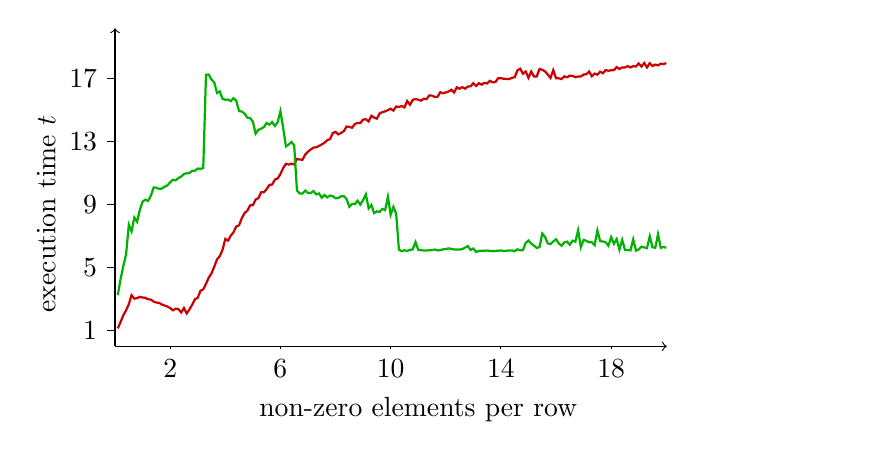
\begin{tikzpicture}[xscale=0.035,yscale=0.2]
  \draw[->] (-0.0,-0.0) -- (200.2,-0.0);
  \draw[->] (0,-0.0) -- (0,20.2);
  \draw (-25,8.4) node[rotate=90] {execution time $t$};

  \foreach \y in {1,5,...,20}
  \draw (0.1,\y) -- (-3,\y) node[anchor=east] {\y};

  %ticks
  \draw (20,-0.0) -- (20,-0.2) node[anchor=north] {2};
  \draw (60,-0.0) -- (60,-0.2) node[anchor=north] {6};
  \draw (100,-0.0) -- (100,-0.2) node[anchor=north] {10};
  \draw (140,-0.0) -- (140,-0.2) node[anchor=north] {14};
  \draw (180,-0.0) -- (180,-0.2) node[anchor=north] {18};

  \draw (110,-4.0) node {non-zero elements per row};

\draw[color=red!80!black,thick] plot[id="newtonjohn"] coordinates {
(  1.0,  1.14) (  2.0,  1.54) ( 3.0,   1.97) (  4.0,  2.29) (  5.0,  2.67) (  6.0,  3.25) (  7.0,  3.03) (  8.0,  3.06) (  9.0,  3.14) ( 10.0,  3.10) 
( 11.0,  3.08) ( 12.0,  2.99) ( 13.0,  2.97) ( 14.0,  2.84) ( 15.0,  2.78) ( 16.0,  2.76) ( 17.0,  2.65) ( 18.0,  2.59) ( 19.0,  2.53) ( 20.0,  2.43) 
( 21.0,  2.29) ( 22.0,  2.39) ( 23.0,  2.37) ( 24.0,  2.15) ( 25.0,  2.43) ( 26.0,  2.09) ( 27.0,  2.35) ( 28.0,  2.65) ( 29.0,  2.99) ( 30.0,  3.08) 
( 31.0,  3.53) ( 32.0,  3.62) ( 33.0,  3.97) ( 34.0,  4.37) ( 35.0,  4.63) ( 36.0,  5.06) ( 37.0,  5.52) ( 38.0,  5.73) ( 39.0,  6.13) ( 40.0,  6.82) 
( 41.0,  6.71) ( 42.0,  7.03) ( 43.0,  7.25) ( 44.0,  7.61) ( 45.0,  7.69) ( 46.0,  8.14) ( 47.0,  8.46) ( 48.0,  8.62) ( 49.0,  8.95) ( 50.0,  8.97) 
( 51.0,  9.32) ( 52.0,  9.41) ( 53.0,  9.78) ( 54.0,  9.78) ( 55.0,  9.98) ( 56.0, 10.25) ( 57.0, 10.27) ( 58.0, 10.59) ( 59.0, 10.66) ( 60.0, 10.94)
( 61.0, 11.32) ( 62.0, 11.59) ( 63.0, 11.54) ( 64.0, 11.60) ( 65.0, 11.55) ( 66.0, 11.90) ( 67.0, 11.86) ( 68.0, 11.85) ( 69.0, 12.18) ( 70.0, 12.36)
( 71.0, 12.50) ( 72.0, 12.62) ( 73.0, 12.64) ( 74.0, 12.72) ( 75.0, 12.82) ( 76.0, 12.93) ( 77.0, 13.09) ( 78.0, 13.16) ( 79.0, 13.54) ( 80.0, 13.62) 
( 81.0, 13.46) ( 82.0, 13.55) ( 83.0, 13.66) ( 84.0, 13.96) ( 85.0, 13.93) ( 86.0, 13.88) ( 87.0, 14.11) ( 88.0, 14.19) ( 89.0, 14.18) ( 90.0, 14.40) 
( 91.0, 14.42) ( 92.0, 14.28) ( 93.0, 14.64) ( 94.0, 14.53) ( 95.0, 14.46) ( 96.0, 14.79) ( 97.0, 14.87) ( 98.0, 14.92) ( 99.0, 15.00) (100.0, 15.09) 
(101.0, 14.97) (102.0, 15.23) (103.0, 15.20) (104.0, 15.26) (105.0, 15.17) (106.0, 15.58) (107.0, 15.34) (108.0, 15.65) (109.0, 15.70) (110.0, 15.66) 
(111.0, 15.60) (112.0, 15.72) (113.0, 15.70) (114.0, 15.93) (115.0, 15.92) (116.0, 15.84) (117.0, 15.84) (118.0, 16.14) (119.0, 16.07) (120.0, 16.12) 
(121.0, 16.18) (122.0, 16.29) (123.0, 16.12) (124.0, 16.45) (125.0, 16.36) (126.0, 16.46) (127.0, 16.36) (128.0, 16.50) (129.0, 16.51) (130.0, 16.71) 
(131.0, 16.53) (132.0, 16.71) (133.0, 16.62) (134.0, 16.73) (135.0, 16.69) (136.0, 16.86) (137.0, 16.77) (138.0, 16.78) (139.0, 17.03) (140.0, 17.03) 
(141.0, 16.99) (142.0, 16.98) (143.0, 16.97) (144.0, 17.05) (145.0, 17.09) (146.0, 17.53) (147.0, 17.63) (148.0, 17.31) (149.0, 17.45) (150.0, 17.05) 
(151.0, 17.45) (152.0, 17.14) (153.0, 17.14) (154.0, 17.61) (155.0, 17.56) (156.0, 17.46) (157.0, 17.26) (158.0, 17.04) (159.0, 17.54) (160.0, 17.02) 
(161.0, 17.02) (162.0, 16.97) (163.0, 17.14) (164.0, 17.09) (165.0, 17.19) (166.0, 17.17) (167.0, 17.09) (168.0, 17.13) (169.0, 17.14) (170.0, 17.26) 
(171.0, 17.28) (172.0, 17.45) (173.0, 17.15) (174.0, 17.32) (175.0, 17.25) (176.0, 17.44) (177.0, 17.34) (178.0, 17.54) (179.0, 17.50) (180.0, 17.53) 
(181.0, 17.54) (182.0, 17.73) (183.0, 17.61) (184.0, 17.71) (185.0, 17.71) (186.0, 17.80) (187.0, 17.71) (188.0, 17.79) (189.0, 17.77) (190.0, 17.96) 
(191.0, 17.77) (192.0, 17.99) (193.0, 17.71) (194.0, 17.98) (195.0, 17.80) (196.0, 17.89) (197.0, 17.84) (198.0, 17.95) (199.0, 17.92) (200.0, 17.99)
} node[right,color=white] {Newton-John};


\draw[color=green!70!black,thick] plot[id="ple"] coordinates {
(  1.0,  3.25) (  2.0, 4.27) (  3.0,  5.09) (  4.0,  5.84) (  5.0,  7.72) (  6.0,  7.30) (  7.0, 8.18) (  8.0,  7.91) (  9.0,  8.66) ( 10.0,  9.19)
( 11.0,  9.32) ( 12.0, 9.23) ( 13.0,  9.57) ( 14.0, 10.09) ( 15.0, 10.07) ( 16.0, 10.00) ( 17.0,10.02) ( 18.0, 10.14) ( 19.0, 10.22) ( 20.0, 10.42)
( 21.0, 10.58) ( 22.0,10.54) ( 23.0, 10.69) ( 24.0, 10.78) ( 25.0, 10.94) ( 26.0, 10.99) ( 27.0,11.00) ( 28.0, 11.15) ( 29.0, 11.15) ( 30.0, 11.29) 
( 31.0, 11.27) ( 32.0,11.32) ( 33.0, 17.25) ( 34.0, 17.26) ( 35.0, 16.94) ( 36.0, 16.76) ( 37.0,16.09) ( 38.0, 16.19) ( 39.0, 15.72) ( 40.0, 15.66) 
( 41.0, 15.67) ( 42.0,15.57) ( 43.0, 15.76) ( 44.0, 15.59) ( 45.0, 14.94) ( 46.0, 14.91) ( 47.0,14.78) ( 48.0, 14.52) ( 49.0, 14.50) ( 50.0, 14.27) 
( 51.0, 13.50) ( 52.0,13.75) ( 53.0, 13.82) ( 54.0, 13.92) ( 55.0, 14.18) ( 56.0, 14.08) ( 57.0,14.24) ( 58.0, 13.99) ( 59.0, 14.23) ( 60.0, 14.93)
( 61.0, 13.86) ( 62.0,12.70) ( 63.0, 12.81) ( 64.0, 12.98) ( 65.0, 12.76) ( 66.0,  9.90) ( 67.0, 9.70) ( 68.0,  9.70) ( 69.0,  9.89) ( 70.0,  9.74)
( 71.0,  9.74) ( 72.0, 9.86) ( 73.0,  9.65) ( 74.0,  9.71) ( 75.0,  9.44) ( 76.0,  9.61) ( 77.0, 9.46) ( 78.0,  9.58) ( 79.0,  9.53) ( 80.0,  9.40)
( 81.0,  9.42) ( 82.0, 9.52) ( 83.0,  9.54) ( 84.0,  9.36) ( 85.0,  8.86) ( 86.0,  9.04) ( 87.0, 9.03) ( 88.0,  9.25) ( 89.0,  9.00) ( 90.0,  9.28) 
( 91.0,  9.65) ( 92.0, 8.76) ( 93.0,  8.97) ( 94.0,  8.46) ( 95.0,  8.57) ( 96.0,  8.54) ( 97.0, 8.73) ( 98.0,  8.65) ( 99.0,  9.49) ( 100.0, 8.36) 
(101.0,  8.86) (102.0, 8.42) (103.0,  6.14) (104.0,  6.04) (105.0,  6.10) (106.0,  6.06) (107.0,  6.13) (108.0, 6.15) (109.0,  6.62) (110.0, 6.13)
(111.0,  6.10) (112.0, 6.09) (113.0,  6.09) (114.0,  6.10) (115.0,  6.11) (116.0,  6.15) (117.0, 6.09) (118.0,  6.11) (119.0,  6.16) (120.0,  6.18)
(121.0,  6.22) (122.0, 6.19) (123.0,  6.15) (124.0,  6.15) (125.0,  6.14) (126.0,  6.18) (127.0, 6.27) (128.0,  6.36) (129.0,  6.12) (130.0,  6.21)
(131.0,  5.99) (132.0,  6.06) (133.0,  6.07) (134.0, 6.07) (135.0,  6.08) (136.0,  6.07) (137.0, 6.04) (138.0,  6.06) (139.0,  6.07) (140.0,  6.09)
(141.0,  6.05) (142.0,  6.07) (143.0, 6.09) (144.0,  6.09) (145.0,  6.04) (146.0,  6.16) (147.0, 6.10) (148.0,  6.11) (149.0,  6.57) (150.0,  6.72)
(151.0,  6.52) (152.0, 6.39) (153.0,  6.25) (154.0,  6.30) (155.0,  7.16) (156.0,  6.95) (157.0, 6.53) (158.0,  6.50) (159.0,  6.66) (160.0,  6.80)
(161.0,  6.54) (162.0, 6.39) (163.0,  6.60) (164.0,  6.65) (165.0,  6.45) (166.0,  6.71) (167.0, 6.65) (168.0,  7.36) (169.0,  6.30) (170.0,  6.76)
(171.0,  6.70) (172.0, 6.61) (173.0,  6.61) (174.0,  6.42) (175.0,  7.36) (176.0,  6.68) (177.0, 6.66) (178.0,  6.61) (179.0,  6.39) (180.0,  6.94)
(181.0,  6.51) (182.0, 6.81) (183.0,  6.14) (184.0,  6.76) (185.0,  6.13) (186.0,  6.12) (187.0, 6.09) (188.0,  6.79) (189.0,  6.08) (190.0,  6.15)
(191.0,  6.33) (192.0, 6.28) (193.0,  6.24) (194.0,  6.99) (195.0,  6.29) (196.0,  6.26) (197.0, 7.12) (198.0,  6.25) (199.0,  6.31) (200.0,  6.26)
} node[right,color=white] {PLE};



\end{tikzpicture}
\caption{Gaussian elimination of $10,000 \times 10,000$ matrices over $\F_{16}$ on 2.67GHz Intel Core i7 M 620.}
\label{fig:sparse-m4rie}
\end{center}
\end{figure}


   
\end{frame}


\begin{frame}{Fin}
\begin{figure}[h]
 \centering
 \includegraphics[width=0.4\textwidth]{./grease.jpg}
 % grease.jpg: 919x1400 pixel, 410dpi, 5.69x8.67 cm, bb=0 0 161 246
\end{figure}

\begin{center}

\end{center}

\end{frame}

\begin{frame}[allowframebreaks]
\bibliographystyle{alpha}
\bibliography{../../literature}
\end{frame}

\end{document}
